\PassOptionsToPackage{unicode=true}{hyperref} % options for packages loaded elsewhere
\PassOptionsToPackage{hyphens}{url}
\PassOptionsToPackage{dvipsnames,svgnames*,x11names*}{xcolor}
%
\documentclass[brazil,]{article}
\usepackage{lmodern}
\usepackage{amssymb,amsmath}
\usepackage{ifxetex,ifluatex}
\usepackage{fixltx2e} % provides \textsubscript
\ifnum 0\ifxetex 1\fi\ifluatex 1\fi=0 % if pdftex
  \usepackage[T1]{fontenc}
  \usepackage[utf8]{inputenc}
  \usepackage{textcomp} % provides euro and other symbols
\else % if luatex or xelatex
  \usepackage{unicode-math}
  \defaultfontfeatures{Ligatures=TeX,Scale=MatchLowercase}
\fi
% use upquote if available, for straight quotes in verbatim environments
\IfFileExists{upquote.sty}{\usepackage{upquote}}{}
% use microtype if available
\IfFileExists{microtype.sty}{%
\usepackage[]{microtype}
\UseMicrotypeSet[protrusion]{basicmath} % disable protrusion for tt fonts
}{}
\IfFileExists{parskip.sty}{%
\usepackage{parskip}
}{% else
\setlength{\parindent}{0pt}
\setlength{\parskip}{6pt plus 2pt minus 1pt}
}
\usepackage{xcolor}
\usepackage{hyperref}
\hypersetup{
            pdftitle={CabotageLens: sistema computacional auditável para comparação porta a porta entre rodovia e cabotagem no Brasil},
            pdfauthor={Felipe de Sá Proença},
            colorlinks=true,
            linkcolor=blue,
            citecolor=Blue,
            urlcolor=blue,
            breaklinks=true}
\urlstyle{same}  % don't use monospace font for urls
\usepackage[margin=2.5cm]{geometry}
\usepackage{color}
\usepackage{fancyvrb}
\newcommand{\VerbBar}{|}
\newcommand{\VERB}{\Verb[commandchars=\\\{\}]}
\DefineVerbatimEnvironment{Highlighting}{Verbatim}{commandchars=\\\{\}}
% Add ',fontsize=\small' for more characters per line
\newenvironment{Shaded}{}{}
\newcommand{\AlertTok}[1]{\textcolor[rgb]{1.00,0.00,0.00}{\textbf{#1}}}
\newcommand{\AnnotationTok}[1]{\textcolor[rgb]{0.38,0.63,0.69}{\textbf{\textit{#1}}}}
\newcommand{\AttributeTok}[1]{\textcolor[rgb]{0.49,0.56,0.16}{#1}}
\newcommand{\BaseNTok}[1]{\textcolor[rgb]{0.25,0.63,0.44}{#1}}
\newcommand{\BuiltInTok}[1]{#1}
\newcommand{\CharTok}[1]{\textcolor[rgb]{0.25,0.44,0.63}{#1}}
\newcommand{\CommentTok}[1]{\textcolor[rgb]{0.38,0.63,0.69}{\textit{#1}}}
\newcommand{\CommentVarTok}[1]{\textcolor[rgb]{0.38,0.63,0.69}{\textbf{\textit{#1}}}}
\newcommand{\ConstantTok}[1]{\textcolor[rgb]{0.53,0.00,0.00}{#1}}
\newcommand{\ControlFlowTok}[1]{\textcolor[rgb]{0.00,0.44,0.13}{\textbf{#1}}}
\newcommand{\DataTypeTok}[1]{\textcolor[rgb]{0.56,0.13,0.00}{#1}}
\newcommand{\DecValTok}[1]{\textcolor[rgb]{0.25,0.63,0.44}{#1}}
\newcommand{\DocumentationTok}[1]{\textcolor[rgb]{0.73,0.13,0.13}{\textit{#1}}}
\newcommand{\ErrorTok}[1]{\textcolor[rgb]{1.00,0.00,0.00}{\textbf{#1}}}
\newcommand{\ExtensionTok}[1]{#1}
\newcommand{\FloatTok}[1]{\textcolor[rgb]{0.25,0.63,0.44}{#1}}
\newcommand{\FunctionTok}[1]{\textcolor[rgb]{0.02,0.16,0.49}{#1}}
\newcommand{\ImportTok}[1]{#1}
\newcommand{\InformationTok}[1]{\textcolor[rgb]{0.38,0.63,0.69}{\textbf{\textit{#1}}}}
\newcommand{\KeywordTok}[1]{\textcolor[rgb]{0.00,0.44,0.13}{\textbf{#1}}}
\newcommand{\NormalTok}[1]{#1}
\newcommand{\OperatorTok}[1]{\textcolor[rgb]{0.40,0.40,0.40}{#1}}
\newcommand{\OtherTok}[1]{\textcolor[rgb]{0.00,0.44,0.13}{#1}}
\newcommand{\PreprocessorTok}[1]{\textcolor[rgb]{0.74,0.48,0.00}{#1}}
\newcommand{\RegionMarkerTok}[1]{#1}
\newcommand{\SpecialCharTok}[1]{\textcolor[rgb]{0.25,0.44,0.63}{#1}}
\newcommand{\SpecialStringTok}[1]{\textcolor[rgb]{0.73,0.40,0.53}{#1}}
\newcommand{\StringTok}[1]{\textcolor[rgb]{0.25,0.44,0.63}{#1}}
\newcommand{\VariableTok}[1]{\textcolor[rgb]{0.10,0.09,0.49}{#1}}
\newcommand{\VerbatimStringTok}[1]{\textcolor[rgb]{0.25,0.44,0.63}{#1}}
\newcommand{\WarningTok}[1]{\textcolor[rgb]{0.38,0.63,0.69}{\textbf{\textit{#1}}}}
\usepackage{longtable,booktabs}
\usepackage{needspace}
% Fix footnotes in tables (requires footnote package)
\IfFileExists{footnote.sty}{\usepackage{footnote}\makesavenoteenv{longtable}}{}
\setlength{\emergencystretch}{3em}  % prevent overfull lines
\providecommand{\tightlist}{%
  \setlength{\itemsep}{0pt}\setlength{\parskip}{0pt}}
\setcounter{secnumdepth}{0}
% Mantém títulos junto do primeiro bloco de conteúdo, evitando títulos órfãos.
\let\oldsection\section
\renewcommand{\section}{\Needspace{14\baselineskip}\oldsection}
\let\oldsubsection\subsection
\renewcommand{\subsection}{\Needspace{12\baselineskip}\oldsubsection}
\let\oldsubsubsection\subsubsection
\renewcommand{\subsubsection}{\Needspace{10\baselineskip}\oldsubsubsection}
% Redefines (sub)paragraphs to behave more like sections
\ifx\paragraph\undefined\else
\let\oldparagraph\paragraph
\renewcommand{\paragraph}[1]{\Needspace{7\baselineskip}\oldparagraph{#1}\mbox{}}
\fi
\ifx\subparagraph\undefined\else
\let\oldsubparagraph\subparagraph
\renewcommand{\subparagraph}[1]{\Needspace{6\baselineskip}\oldsubparagraph{#1}\mbox{}}
\fi

% set default figure placement to htbp
\makeatletter
\def\fps@figure{htbp}
\makeatother

\ifnum 0\ifxetex 1\fi\ifluatex 1\fi=0 % if pdftex
  \usepackage[shorthands=off,main=brazil]{babel}
\else
  % load polyglossia as late as possible as it *could* call bidi if RTL lang (e.g. Hebrew or Arabic)
  \usepackage{polyglossia}
  \setmainlanguage[]{brazil}
\fi
\usepackage[backend=biber,style=abnt,sorting=nyt]{biblatex}
\addbibresource{references.bib}

\title{CabotageLens: sistema computacional auditável para comparação porta a
porta entre rodovia e cabotagem no Brasil}
\author{Felipe de Sá Proença}
\date{}


% -----------------------------------------------------------------------------
% Fonte LaTeX da versão final do artigo técnico.
% O Markdown homônimo mantém a versão em texto simples.
% Compilação prevista: XeLaTeX com Biber.
% -----------------------------------------------------------------------------
\usepackage{tikz}
\usetikzlibrary{arrows.meta,positioning}
\usepackage{listings}
\usepackage{adjustbox}
\definecolor{clblue}{RGB}{32,68,112}
\definecolor{clgray}{RGB}{245,247,250}
\tikzset{
  clnode/.style={draw=clblue!80!black, fill=clgray, rounded corners=3pt,
    align=center, text width=2.35cm, minimum height=0.8cm, inner sep=4pt,
    font=\small},
  clarrow/.style={-{Latex[length=2mm]}, thick, draw=clblue!80!black}
}
\lstset{basicstyle=\ttfamily\small, breaklines=true, frame=single,
  columns=fullflexible, backgroundcolor=\color{clgray}}
\setlength{\emergencystretch}{2em}
\setcounter{secnumdepth}{-\maxdimen}
\setcounter{tocdepth}{4}
\renewcommand{\contentsname}{Sumário}
\renewcommand{\refname}{Referências}

\begin{document}
\maketitle
\thispagestyle{empty}
\clearpage

\tableofcontents
\clearpage

\section*{Dicionário de termos}
\addcontentsline{toc}{section}{Dicionário de termos}

\begin{longtable}{@{}p{0.28\linewidth}p{0.66\linewidth}@{}}
\toprule
\textbf{Termo ou sigla} & \textbf{Significado no estudo} \\
\midrule
\endhead
ANP & Agência Nacional do Petróleo, Gás Natural e Biocombustíveis; publica os preços de Diesel S10 usados no cálculo de custo. \\
ANTAQ & Agência Nacional de Transportes Aquaviários; fornece os registros observados de atracação e movimentação de carga. \\
ANTT & Agência Nacional de Transportes Terrestres; publica os rendimentos rodoviários por número de eixos usados na estimativa de consumo. \\
Cabotagem & Transporte aquaviário de cargas entre portos do mesmo país. \\
CO\textsubscript{2}e & Dióxido de carbono equivalente; unidade que expressa emissões de gases de efeito estufa em uma mesma base. \\
EU MRV & Sistema europeu de Monitoramento, Reporte e Verificação; fornece indicadores anuais de atividade e consumo dos navios. \\
\textit{First mile} e \textit{last mile} & Acessos rodoviários entre a origem e o porto de embarque, e entre o porto de desembarque e o destino, respectivamente. \\
Geocodificação & Conversão de um endereço ou local informado em coordenadas geográficas. \\
Distância de Haversine & Distância geométrica entre dois pontos calculada a partir de latitude e longitude; usada somente para selecionar os portos mais próximos. \\
IMO & Número de identificação permanente atribuído pela Organização Marítima Internacional a cada navio. \\
Intensidade marítima & Combustível associado ao transporte de uma tonelada por uma milha náutica, expresso em g/(t·nm). \\
LCA & \textit{Life-cycle assessment}, ou avaliação de ciclo de vida; fronteira mais ampla que pode incluir veículos, infraestrutura e cadeia do combustível. \\
P95 & Percentil 95; limite usado para identificar valores excepcionalmente altos em conjuntos de dados. \\
Perna marítima & Trecho de cabotagem entre o porto de embarque e o porto de desembarque. \\
TEU e TKU & Unidade equivalente a um contêiner de 20 pés e tonelada-quilômetro útil, respectivamente. \\
Trabalho de transporte & Produto da carga a bordo pela distância em cada subtrecho, expresso em t·nm. \\
TTW e WTW & \textit{Tank-to-wheel}, que considera a queima do combustível durante o transporte, e \textit{well-to-wheel}, que também inclui suas etapas anteriores. \\
VLSFO & \textit{Very low sulphur fuel oil}, óleo combustível naval de baixíssimo teor de enxofre. \\
\bottomrule
\end{longtable}

\clearpage

\hypertarget{introduuxe7uxe3o}{%
\section{1. Introdução}\label{introduuxe7uxe3o}}

O transporte de cargas no Brasil é fortemente concentrado nas rodovias.
Em 2015, o modal rodoviário respondeu por 65\% da atividade de
transporte de cargas, medida em toneladas-quilômetro úteis (TKU). No
mesmo recorte, a ferrovia respondeu por 15\% e a cabotagem por 11\%. A
distribuição ajuda a explicar por que o caminhão é a referência mais
imediata para transportar cargas no país, inclusive em trajetos longos.

\begin{center}
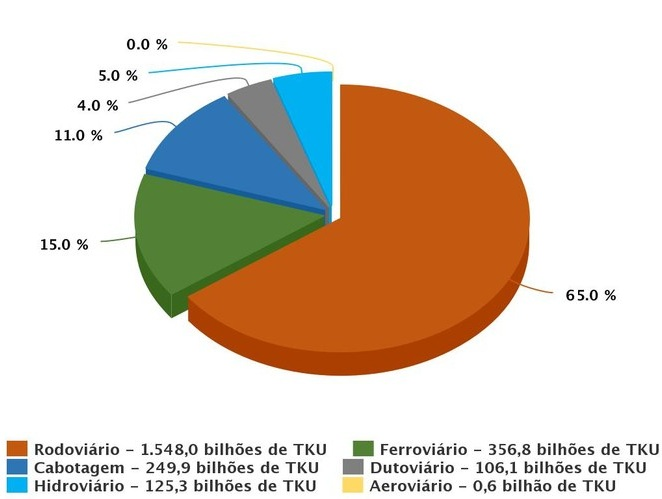
\includegraphics[width=0.94\linewidth]{images/grafico da atividade modal do transporte no Brasil em 2015.jpeg}
\end{center}

\emph{Figura 1 --- Distribuição da atividade de transporte de cargas no
Brasil em 2015, medida em TKU. Fonte:
\textcite{spbancarios2018}, com dados de 2015
do Plano Nacional de Logística, conforme informado pela publicação.}

Além do papel predominante na matriz, o transporte rodoviário de cargas
depende, principalmente, do diesel e contribui para as emissões de gases
de efeito estufa do setor. Por isso, políticas de transporte buscam
transferir parte das viagens longas para modais mais eficientes. Tomemos
de exemplo a
\href{https://eur-lex.europa.eu/legal-content/EN/TXT/?uri=CELEX:52011DC0144}{Comissão
Europeia}, que no Livro Branco dos Transportes definiu a meta de
transferir, até 2030, 30\% das cargas rodoviárias transportadas por mais
de 300 km para ferrovias ou vias aquaviárias e, até 2050, mais de 50\%
\parencite{eupolicy2011}.
Nesse contexto, a cabotagem --- o transporte marítimo entre portos do
mesmo país utilizando a navegação pela costa nacional ou por vias
interiores --- é uma alternativa possível para parte das cargas de longa
distância no Brasil \parencite{icct2022}.

Para saber se a cabotagem faz sentido em uma ligação específica, a
comparação precisa ser porta a porta. Uma comparação porta a porta
começa no local onde a carga está e termina no local em que ela será
entregue. As duas alternativas precisam prestar exatamente o mesmo
serviço: transportar a mesma massa entre esses dois pontos. No caminho
rodoviário, o caminhão percorre todo o trajeto por estrada. Na
alternativa com cabotagem, a carga segue de caminhão até o porto de
embarque, é transportada pelo navio entre os portos e, em seguida, segue
de caminhão do porto de desembarque até o destino final. Por isso, a
análise soma distância, consumo, emissões e custo de todas essas etapas,
em vez de comparar apenas o trecho marítimo com a viagem rodoviária
completa. Os portos escolhidos, as distâncias de acesso, a carga e as
operações de transbordo podem mudar o resultado
\parencite{shortsea2019,modalshiftreview2020}.

É para tornar essa comparação possível que foi desenvolvido o
CabotageLens. O usuário informa a origem, o destino e a massa da carga,
e o sistema constrói as duas alternativas de transporte. Para cada uma,
apresenta a distância total, o consumo de combustível, as emissões
operacionais e o custo modelado do combustível. Ao reunir essas
informações em uma mesma base de comparação, a ferramenta permite
avaliar, para cada ligação, como a alternativa com cabotagem se
diferencia da rota feita inteiramente por estrada. Com isso, a
comparação deixa de ser uma escolha abstrata entre caminhão e navio e
passa a considerar a operação logística completa.

\hypertarget{revisuxe3o-da-literatura-e-fundamentauxe7uxe3o-metodoluxf3gica}{%
\section{2. Revisão da literatura e fundamentação
metodológica}\label{revisuxe3o-da-literatura-e-fundamentauxe7uxe3o-metodoluxf3gica}}

A literatura mostra que a cabotagem pode ser relevante em viagens
longas, mas o resultado muda de uma ligação para outra \parencite{icct2022}.
Uma rota pode ter uma longa navegação e acessos rodoviários curtos.
Outra pode exigir muitos quilômetros por estrada até o porto.
Frequência, tempo, confiabilidade, estoque e disponibilidade do serviço
também influenciam a decisão real \parencite{competitiveness2024}. O
CabotageLens calcula rotas, combustível, emissões operacionais e custo
modelado do combustível. Ele não representa por completo todas as
condições comerciais.

Estudos de \emph{short sea shipping} (navegação marítima de curta
distância) também mostram que a substituição do transporte rodoviário
pelo transporte marítimo não significa uma vantagem ambiental
automática. O resultado depende do tipo de navio, de sua utilização, das
distâncias e da carga à qual o consumo é atribuído \parencite{shortsea2019}.
Por isso, a unidade analisada deve ser a remessa completa, e não um
navio e um caminhão considerados isoladamente
\parencite{modalshiftreview2020}.

Um princípio metodológico do estudo é dar preferência a dados públicos,
oficiais, observados e auditáveis. A Agência Nacional de Transportes
Aquaviários (ANTAQ), órgão federal que regula e acompanha o transporte
aquaviário brasileiro, fornece os registros de escalas e de movimentação
de carga. A base europeia de Monitoramento, Reporte e Verificação da
União Europeia (EU MRV) publica indicadores anuais de consumo e
atividade dos navios. Essas fontes permitem relacionar uma operação
registrada no Brasil ao desempenho do navio identificado pelo número da
Organização Marítima Internacional (IMO), uma identificação permanente
da embarcação. Os campos utilizados, os arquivos de origem e a forma de
reconstruir as viagens são apresentados na Seção 3.3
\parencite{antaq2025,emsa2026}.

O cálculo de emissões adota a fronteira operacional \emph{tank-to-wheel}
(TTW, do tanque à roda), pois o objetivo é comparar as emissões
diretamente associadas ao transporte da mesma remessa. Em um caminhão a
diesel, por exemplo, isso corresponde às emissões liberadas pelo
escapamento durante a viagem. As fronteiras \emph{well-to-wheel} (WTW,
do poço à roda) e de avaliação de ciclo de vida (\emph{life-cycle
assessment}, LCA) ampliariam a análise para etapas que ocorrem antes ou
além do deslocamento \parencite{decarb2024,maritimelca2024}, mas não foram
adotadas no presente estudo.

\textbf{Quadro 1 --- Fronteiras de emissão e aplicação ao caminhão a
diesel.}

\begin{longtable}[]{@{}lll@{}}
\toprule
\begin{minipage}[b]{0.30\columnwidth}\raggedright
Fronteira\strut
\end{minipage} & \begin{minipage}[b]{0.30\columnwidth}\raggedright
Conceito\strut
\end{minipage} & \begin{minipage}[b]{0.30\columnwidth}\raggedright
Aplicação prática ao caminhão\strut
\end{minipage}\tabularnewline
\midrule
\endhead
\begin{minipage}[t]{0.30\columnwidth}\raggedright
TTW (\emph{tank-to-wheel})\strut
\end{minipage} & \begin{minipage}[t]{0.30\columnwidth}\raggedright
Considera somente a queima do combustível durante o transporte.\strut
\end{minipage} & \begin{minipage}[t]{0.30\columnwidth}\raggedright
Emissões do escapamento ao longo da viagem.\strut
\end{minipage}\tabularnewline
\begin{minipage}[t]{0.30\columnwidth}\raggedright
WTW (\emph{well-to-wheel})\strut
\end{minipage} & \begin{minipage}[t]{0.30\columnwidth}\raggedright
Inclui a queima e as etapas anteriores da cadeia do combustível.\strut
\end{minipage} & \begin{minipage}[t]{0.30\columnwidth}\raggedright
Também inclui extração, refino, transporte e distribuição do
diesel.\strut
\end{minipage}\tabularnewline
\begin{minipage}[t]{0.30\columnwidth}\raggedright
LCA (\emph{life-cycle assessment})\strut
\end{minipage} & \begin{minipage}[t]{0.30\columnwidth}\raggedright
Avalia um escopo mais amplo do sistema de transporte.\strut
\end{minipage} & \begin{minipage}[t]{0.30\columnwidth}\raggedright
Pode incluir a fabricação, a manutenção e o fim de vida do caminhão e da
infraestrutura.\strut
\end{minipage}\tabularnewline
\bottomrule
\end{longtable}

\emph{Fonte: elaboração própria com base em
\parencite{decarb2024,maritimelca2024}.}

Além das emissões, o estudo delimita o custo e o serviço que serão
comparados. O custo apresentado é uma estimativa do custo do combustível
consumido nas etapas calculadas. Ele não representa frete comercial,
tarifa contratada, negociação, seguro, estoque ou multas por
permanência. O serviço comparado é o transporte da mesma remessa entre a
mesma origem e o mesmo destino. As viagens observadas permitem
reconstruir os percursos marítimos, mas não garantem frequência, espaço
no navio ou disponibilidade comercial futura.

\textbf{Tabela 1 --- O que está dentro e fora da comparação.}

\begin{longtable}[]{@{}lll@{}}
\toprule
\begin{minipage}[b]{0.07\columnwidth}\raggedright
Dimensão\strut
\end{minipage} & \begin{minipage}[b]{0.39\columnwidth}\raggedright
Incluído\strut
\end{minipage} & \begin{minipage}[b]{0.45\columnwidth}\raggedright
Não incluído no cálculo\strut
\end{minipage}\tabularnewline
\midrule
\endhead
\begin{minipage}[t]{0.07\columnwidth}\raggedright
Emissões\strut
\end{minipage} & \begin{minipage}[t]{0.39\columnwidth}\raggedright
Emissões operacionais TTW de CO\textsubscript{2}e por remessa\strut
\end{minipage} & \begin{minipage}[t]{0.45\columnwidth}\raggedright
WTW, LCA, fabricação de caminhões, navios e equipamentos portuários e
inventário completo de poluentes locais\strut
\end{minipage}\tabularnewline
\begin{minipage}[t]{0.07\columnwidth}\raggedright
Custo\strut
\end{minipage} & \begin{minipage}[t]{0.39\columnwidth}\raggedright
Estimativa do custo modelado do combustível\strut
\end{minipage} & \begin{minipage}[t]{0.45\columnwidth}\raggedright
Frete comercial, negociação, seguro, estoque, multas por permanência e
reserva de espaço no navio\strut
\end{minipage}\tabularnewline
\begin{minipage}[t]{0.07\columnwidth}\raggedright
Serviço\strut
\end{minipage} & \begin{minipage}[t]{0.39\columnwidth}\raggedright
Sequências de portos realmente registradas no período analisado\strut
\end{minipage} & \begin{minipage}[t]{0.45\columnwidth}\raggedright
Garantia de frequência, espaço no navio ou disponibilidade comercial
futura\strut
\end{minipage}\tabularnewline
\bottomrule
\end{longtable}

\hypertarget{metodologia}{%
\section{3. Metodologia}\label{metodologia}}

Esta seção descreve como o CabotageLens constrói e compara as
alternativas de transporte. A Seção 3.1 define o serviço que as duas
alternativas precisam atender. Em seguida, a Seção 3.2 calcula a
alternativa rodoviária e a Seção 3.3 monta a alternativa com cabotagem,
incluindo os acessos terrestres, as operações portuárias e a navegação.
A Seção 3.4 reúne os resultados do exemplo. A Seção 4 apresenta a
implementação dessas regras no sistema.

\hypertarget{serviuxe7o-comparado-e-alternativas-loguxedsticas}{%
\subsection{3.1 Serviço comparado e alternativas
logísticas}\label{serviuxe7o-comparado-e-alternativas-loguxedsticas}}

Para que a comparação seja válida, as duas alternativas devem prestar o
mesmo serviço: entregar uma remessa com massa definida entre a mesma
origem e o mesmo destino. Esses três elementos formam a unidade
funcional da avaliação. Assim, uma alternativa não pode apresentar
resultado mais favorável apenas por transportar menos carga ou terminar
em outro local.

Nos exemplos desta seção, a remessa tem 14~t e segue de São Paulo (SP)
para Rio Branco (AC). Na alternativa rodoviária, ela percorre um único
trecho por estrada, da origem ao destino. Na alternativa com cabotagem,
a mesma remessa percorre três trechos:

\begin{itemize}
\tightlist
\item
  origem → porto de embarque;
\item
  porto de embarque → porto de desembarque; e
\item
  porto de desembarque → destino.
\end{itemize}

As operações de movimentação de carga nos dois terminais também entram
no cálculo. Dessa forma, a comparação considera a cadeia completa, e não
apenas o trecho marítimo frente à viagem rodoviária inteira
\parencite{shortsea2019,competitiveness2024}.

Para estimar as operações portuárias, o sistema representa a remessa de
14~t como 1~TEU (\emph{twenty-foot equivalent unit}, unidade equivalente
a um contêiner de 20 pés). Essa conversão determina quantos contêineres
precisam ser movimentados nos terminais.

\textbf{Quadro 2 --- Principais símbolos usados nas fórmulas do
sistema.}

\begin{longtable}[]{@{}lll@{}}
\toprule
Grandeza & Símbolo & Unidade usual\tabularnewline
\midrule
\endhead
Distância & \(D\) & km ou milhas náuticas (nm)\tabularnewline
Volume de diesel & \(V\) & L\tabularnewline
Massa de VLSFO (óleo combustível naval de baixo teor de enxofre) & \(M\)
& kg\tabularnewline
Massa da carga & \(m\) & t\tabularnewline
Preço do combustível & \(P\) & R\(/L ou R\)/kg\tabularnewline
Custo modelado do combustível & \(C\) & R\$\tabularnewline
Emissão operacional & \(E\) & kg CO\textsubscript{2}e\tabularnewline
Fator de emissão & \(FE\) & kg CO\textsubscript{2}e/L\tabularnewline
Eficiência do veículo & \(\eta\) & km/L\tabularnewline
Intensidade marítima & \(I\) & g/(t·nm)\tabularnewline
Trabalho de transporte & \(W\) & t·nm\tabularnewline
Quantidade contável & \(N\) & viagens, TEUs ou recortes\tabularnewline
Movimentos por TEU & \(a\) & movimentos/TEU\tabularnewline
Consumo por movimento & \(c\) & L/movimento\tabularnewline
\bottomrule
\end{longtable}

\emph{Os subscritos identificam a etapa, o combustível ou o conjunto de
dados. Os índices e conjuntos específicos são definidos junto às
fórmulas em que aparecem.}

\hypertarget{alternativa-rodoviuxe1ria}{%
\subsection{3.2 Alternativa
rodoviária}\label{alternativa-rodoviuxe1ria}}

O cálculo rodoviário começa pela distância terrestre total entre a
origem e o destino. O sistema obtém uma rota rodoviária em quilômetros e
utiliza essa distância para representar o percurso do caminhão. A forma
como essa rota é consultada e transformada em distância está descrita na
Seção~4.3.1.

\hypertarget{escolha-do-veuxedculo-e-consumo-de-diesel}{%
\subsubsection{3.2.1 Escolha do veículo e consumo de
diesel}\label{escolha-do-veuxedculo-e-consumo-de-diesel}}

A massa transportada define o veículo representativo. O modelo utiliza
os rendimentos médios por número de eixos publicados pela
\textbf{Agência Nacional de Transportes Terrestres (ANTT)}. Esses dados
oficiais foram obtidos na tabela da Política Nacional de Pisos Mínimos
do Transporte Rodoviário de Cargas, disponibilizada no
\href{https://anttlegis.antt.gov.br/action/UrlPublicasAction.php?acao=abrirAtoPublico\&cod_menu=9230\&cod_modulo=623\&num_ato=00000001\&seq_ato=ATT\&sgl_orgao=SUROC\%2FANTT\%2FMT\&sgl_tipo=POR\&vlr_ano=2025}{portal
de legislação da ANTT (ANTTlegis)} \parencite{antt2025}. A tabela de referência adotada no
modelo associa a faixa de carga ao número de eixos e relaciona cada
configuração à eficiência básica em quilômetros por litro (km/L). A
seleção automática é uma regra de modelagem para estimar consumo; não é
uma verificação de limite legal de peso nem substitui o planejamento
operacional de uma transportadora.

\textbf{Tabela 2 --- Regra automática para o veículo rodoviário
representativo e eficiência básica adotada.}

\begin{longtable}[]{@{}llrr@{}}
\toprule
Massa da remessa & Veículo representativo & Eixos & Eficiência
básica\tabularnewline
\midrule
\endhead
Até 18~t & Carreta & 5 & 2,3~km/L\tabularnewline
Acima de 18~t até 30~t & Carreta & 6 & 2,0~km/L\tabularnewline
Acima de 30~t até 40~t & Bitrem & 7 & 2,0~km/L\tabularnewline
Acima de 40~t & Rodotrem & 9 & 2,0~km/L\tabularnewline
\bottomrule
\end{longtable}

\emph{Fonte: elaboração do sistema a partir dos rendimentos médios por
número de eixos publicados pela Agência Nacional de Transportes
Terrestres (ANTT), no portal ANTTlegis.}

Com a distância rodoviária \(D_{\mathrm{rod}}\), em quilômetros, a
eficiência aplicada \(\eta_{\mathrm{rod}}\), em km/L, e
\(N_{\mathrm{viagens}}\) viagens carregadas necessárias para transportar
a remessa, o volume de diesel do trecho \(V_{\mathrm{diesel,rod}}\) é
calculado por:

\[
V_{\mathrm{diesel,rod}}
=N_{\mathrm{viagens}}\frac{D_{\mathrm{rod}}}{\eta_{\mathrm{rod}}}.
\]

Como exemplo, usemos os 3.491,431~km de distância rodoviária entre São
Paulo e Rio Branco. Para transportar uma remessa de 14~t nessa ligação,
o modelo seleciona uma carreta de cinco eixos, com eficiência de
2,3~km/L. Como a remessa cabe em uma única viagem,
\(N_{\mathrm{viagens}}=1\) e o consumo estimado é:

\[
\begin{aligned}
V_{\mathrm{diesel,rod}}
&=1\times\frac{3.491{,}431\ \mathrm{km}}{2{,}3\ \mathrm{km/L}}\\
&=1.518{,}014\ \mathrm{L}.
\end{aligned}
\]

Quando a carga exige mais de uma viagem do veículo escolhido, o sistema
multiplica esse consumo pelo número necessário de viagens carregadas. Os
litros calculados são convertidos em custo na Seção~3.2.2 e em emissões
operacionais na Seção~3.2.3.

\hypertarget{custo-estimado-do-combustuxedvel}{%
\subsubsection{3.2.2 Custo estimado do
combustível}\label{custo-estimado-do-combustuxedvel}}

Após estimar o consumo em litros, o sistema calcula o custo do diesel da
rota rodoviária. O preço do Diesel S10 vem do levantamento semanal da
\href{https://www.gov.br/anp/pt-br/assuntos/precos-e-defesa-da-concorrencia/precos/levantamento-de-precos-de-combustiveis-ultimas-semanas-pesquisadas}{Agência
Nacional do Petróleo, Gás Natural e Biocombustíveis (ANP)}, agência
federal que publica preços médios de combustíveis por Unidade da
Federação (UF) \parencite{anp2026}. O sistema sempre busca os dados mais recentes para a
comparação.

Nas rotas interestaduais, o preço adotado é a média aritmética entre o
valor registrado na UF de origem e o valor registrado na UF de destino.
Em uma rota inteiramente dentro de uma mesma UF, os dois valores são
iguais e, portanto, o cálculo mantém o preço desse estado. O preço usado
na rota é dado por:

\[
P_{\mathrm{diesel}}
=\frac{P_{\mathrm{diesel,origem}}+P_{\mathrm{diesel,destino}}}{2}.
\]

O custo estimado é o consumo calculado na Seção 3.2.1 multiplicado pelo
preço do litro:

\[
C_{\mathrm{rod}}=V_{\mathrm{diesel,rod}}\,P_{\mathrm{diesel}}.
\]

Nessas expressões, \(C_{\mathrm{rod}}\) é o custo modelado do
combustível da rota, em reais; \(V_{\mathrm{diesel,rod}}\) é o volume de
diesel, em litros; e \(P_{\mathrm{diesel}}\) é o preço adotado, em reais
por litro. \(P_{\mathrm{diesel,origem}}\) e
\(P_{\mathrm{diesel,destino}}\) são, respectivamente, os preços do
Diesel S10 nas Unidades da Federação de origem e destino. Na execução
São Paulo--Rio Branco, os valores correspondem aos preços médios de
revenda do Diesel S10 divulgados pela ANP para a semana de 12 a 18 de
julho de 2026. Nesse levantamento, São Paulo registrou R\$~6,960/L e o
Acre, R\$~9,270/L. Assim, o preço aplicado à rota foi:

\[
P_{\mathrm{diesel}}
=\frac{6{,}960+9{,}270}{2}
=8{,}115\ \text{R\$/L}.
\]

Com o consumo de 1.518,014~L calculado para a remessa de 14~t, o custo
estimado da rota rodoviária é:

\[
\begin{aligned}
C_{\mathrm{rod}}
&=V_{\mathrm{diesel,rod}}\times P_{\mathrm{diesel}}\\
&=1.518{,}014\ \mathrm{L}\times8{,}115\ \text{R\$/L}\\
&=12.318{,}68\ \text{R\$}.
\end{aligned}
\]

\hypertarget{emissuxf5es-operacionais-da-perna-rodoviuxe1ria}{%
\subsubsection{3.2.3 Emissões operacionais da perna
rodoviária}\label{emissuxf5es-operacionais-da-perna-rodoviuxe1ria}}

As emissões da alternativa rodoviária são calculadas a partir do diesel
consumido na Seção~3.2.1. A fronteira adotada é \emph{tank-to-wheel}
(TTW, do tanque à roda): ela considera somente as emissões geradas pela
queima do combustível durante o transporte. O sistema aplica o fator
2,68~kg~CO\textsubscript{2}e por litro de diesel, baseado nas Diretrizes de 2006 do
Painel Intergovernamental sobre Mudanças Climáticas (IPCC)
\parencite{ipcc2006}. \textcite{competitiveness2024} é a referência
brasileira usada para manter essa estimativa na fronteira TTW, sem
incluir a produção, o refino ou a distribuição do combustível.

A emissão rodoviária é o consumo de diesel multiplicado pelo fator de
emissão:

\[
E_{\mathrm{rod}}
=V_{\mathrm{diesel,rod}}\,FE_{\mathrm{diesel}}.
\]

Nessa expressão, \(E_{\mathrm{rod}}\) é a emissão operacional da rota,
em kg~CO\textsubscript{2}e; \(V_{\mathrm{diesel,rod}}\) é o volume de diesel, em litros;
e \(FE_{\mathrm{diesel}}\) é o fator de emissão, em kg~CO\textsubscript{2}e/L. No
exemplo São Paulo--Rio Branco, os 1.518,014~L estimados na Seção~3.2.1
resultam em:

\[
\begin{aligned}
E_{\mathrm{rod}}
&=V_{\mathrm{diesel,rod}}\times FE_{\mathrm{diesel}}\\
&=1.518{,}014\ \mathrm{L}\times2{,}68\ \text{kg CO\textsubscript{2}e/L}\\
&=4.068{,}28\ \text{kg CO\textsubscript{2}e}.
\end{aligned}
\]

\hypertarget{resultado-consolidado-da-alternativa-rodoviuxe1ria}{%
\subsubsection{3.2.4 Resultado consolidado da alternativa
rodoviária}\label{resultado-consolidado-da-alternativa-rodoviuxe1ria}}

A Tabela 3 reúne os resultados da alternativa rodoviária para a mesma
remessa usada no exemplo São Paulo-Rio Branco.

\textbf{Tabela 3 --- Resultados da alternativa rodoviária no exemplo São
Paulo--Rio Branco, para uma remessa de 14~t.}

\begin{longtable}[]{@{}ll@{}}
\toprule
Item & Valor no exemplo\tabularnewline
\midrule
\endhead
\textbf{Percurso} & São Paulo (SP)--Rio Branco (AC)\tabularnewline
\textbf{Distância rodoviária} & 3.491,431~km\tabularnewline
\textbf{Veículo representativo} & Carreta de cinco eixos\tabularnewline
\textbf{Eficiência adotada} & 2,3~km/L\tabularnewline
\textbf{Número de viagens carregadas} & 1\tabularnewline
\textbf{Diesel consumido} & 1.518,014~L\tabularnewline
\textbf{Preço do Diesel S10} & R\$~8,115/L\tabularnewline
\textbf{Custo modelado do combustível} & R\$~12.318,68\tabularnewline
\textbf{Emissões operacionais TTW} & 4.068,28~kg~CO\textsubscript{2}e\tabularnewline
\bottomrule
\end{longtable}

\hypertarget{alternativa-multimodal}{%
\subsection{3.3 Alternativa multimodal}\label{alternativa-multimodal}}

A alternativa multimodal também precisa transportar a remessa do ponto
inicial ao ponto final. Ela é formada por três partes: o acesso
rodoviário até o porto de embarque, a navegação entre os portos e o
acesso rodoviário após o desembarque. Portanto, o combustível é
consumido não só pelo navio, em cada subtrecho marítimo, mas também nos
deslocamentos da origem até o porto de embarque e do porto de
desembarque até o destino final. Além disso, o sistema calcula
separadamente o consumo da movimentação de carga nos terminais
portuários.

Os próximos subitens mostram como esses componentes são formados: a
escolha dos portos define os extremos da ligação; os acessos terrestres
usam o cálculo rodoviário; as viagens registradas permitem reconstruir a
navegação e a carga a bordo; a intensidade define o consumo do navio; e
a agregação reúne combustível, emissões, custo e operações portuárias.

\hypertarget{escolha-dos-portos}{%
\subsubsection{3.3.1 Escolha dos portos}\label{escolha-dos-portos}}

O sistema associa a origem ao porto mais próximo disponível na base
portuária e faz o mesmo para o destino. Esses dois portos definem a
ligação marítima que será pesquisada. A forma como essa proximidade é
calculada e usada para selecionar os portos é apresentada na
Seção~4.4.3.1. Essa regra fornece uma forma objetiva de montar o
cenário, mas não afirma se o porto é necessariamente a melhor escolha
comercial ou operacional. Um porto mais distante pode ser preferível na
prática por motivos como frequência de navios, contrato, terminal, custo
ou disponibilidade de espaço, fatores que não são decididos por essa
seleção geográfica.

\hypertarget{acessos-rodoviuxe1rios-first-mile-e-last-mile}{%
\subsubsection{\texorpdfstring{3.3.2 Acessos rodoviários: \emph{first
mile} e \emph{last
mile}}{3.3.2 Acessos rodoviários: first mile e last mile}}\label{acessos-rodoviuxe1rios-first-mile-e-last-mile}}

O primeiro acesso, chamado de \emph{first mile}, leva a carga da origem
até o porto de embarque. O segundo, chamado de \emph{last mile}, leva a
carga do porto de desembarque até o destino final. Para cada um deles, o
sistema obtém uma distância rodoviária, aplica a regra de veículo,
eficiência e consumo de diesel da Seção~3.2.1 e converte o consumo em
emissões conforme a Seção~3.2.3.

\hypertarget{operauxe7uxf5es-portuuxe1rias}{%
\subsubsection{3.3.3 Operações
portuárias}\label{operauxe7uxf5es-portuuxe1rias}}

As operações portuárias são as movimentações realizadas dentro do
terminal quando a remessa passa entre o transporte rodoviário e o navio.
No porto de embarque, o contêiner chega pelo \emph{first mile} e precisa
ser movimentado até o navio; no porto de desembarque, ocorre o caminho
inverso antes do \emph{last mile}. Essas atividades não pertencem nem ao
acesso rodoviário nem à navegação. Por isso, o combustível consumido no
terminal é calculado como um componente próprio da alternativa
multimodal.

O modelo representa esse consumo pelos equipamentos para os quais há
fatores de atividade no cenário adotado: o guindaste sobre pneus do
pátio (\emph{rubber-tyred gantry}, RTG) e o caminhão que circula
internamente no terminal. Estudos sobre carga e descarga em portos e
sobre o uso energético de RTGs fundamentam a representação da operação
por equipamento a seguir \parencite{shipops2022,rtg2017}.

O cálculo segue uma sequência simples: a carga informada é convertida em
contêineres equivalentes a 20 pés (TEU); cada TEU gera uma quantidade
definida de movimentos por equipamento; e cada movimento é convertido em
litros de diesel. Os movimentos por contêiner e os consumos por
movimento vêm do cenário de referência parametrizado com dados de Santos
\parencite{workbookdados}.

O cenário sempre considera duas operações portuárias: uma no porto de
embarque e outra no porto de desembarque. Como a mesma remessa passa
pelos dois terminais, a fórmula já usa a multiplicação por 2:

\[
V_{\mathrm{diesel,porto}}
=2\times N_{\mathrm{TEU}}\times
\left(a_{\mathrm{RTG}}\times\,c_{\mathrm{RTG}}
+a_{\mathrm{caminhao}}\times\,c_{\mathrm{caminhao}}\right).
\]

Nessa expressão, \(V_{\mathrm{diesel,porto}}\) é o volume total de
diesel das duas operações portuárias, em litros; \(N_{\mathrm{TEU}}\) é
a quantidade de TEUs da remessa; \(a\) é o número de movimentos por TEU;
e \(c\) é o consumo de diesel, em litros por movimento. O primeiro termo
(\(a_{\mathrm{RTG}}\times\,c_{\mathrm{RTG}}\)) calcula o diesel do RTG e
o segundo (\(a_{\mathrm{caminhao}}\times\,c_{\mathrm{caminhao}}\))
calcula o diesel do caminhão interno. A multiplicação por 2 leva esse
consumo para os dois terminais. O resultado é usado posteriormente no
cálculo das emissões operacionais e do custo modelado do combustível.

No exemplo, a remessa de 14~t equivale a 1~TEU. O RTG realiza quatro
movimentos por contêiner, com consumo de 0,355148~L por movimento, e o
caminhão interno realiza dois movimentos, com consumo de 0,494671~L por
movimento. Aplicando diretamente a fórmula:

\[
\begin{aligned}
V_{\mathrm{diesel,porto}}
&=2\times1\times
\left[(4\times0{,}355148)+(2\times0{,}494671)\right]\\
&=2\times(1{,}421+0{,}989)\\
&=4{,}820\ \mathrm{L}.
\end{aligned}
\]

Assim, no exemplo São Paulo--Rio Branco, as operações portuárias em
Santos e Manaus totalizam 4,820~L de diesel.

\hypertarget{consumo-de-combustuxedvel-na-perna-maruxedtima}{%
\subsubsection{3.3.4 Consumo de combustível na perna
marítima}\label{consumo-de-combustuxedvel-na-perna-maruxedtima}}

A perna marítima corresponde ao deslocamento da remessa por cabotagem
entre o porto de embarque e o porto de desembarque. Nesta etapa, o modelo
estima o consumo de VLSFO (\emph{very low sulphur fuel oil}, óleo
combustível de baixíssimo teor de enxofre) associado a esse deslocamento.

A estimativa não parte de um corredor previamente definido. Ela é
construída com registros observados de escalas e movimentações de carga
da Agência Nacional de Transportes Aquaviários (ANTAQ) e com indicadores
de intensidade de combustível do Monitoramento, Reporte e Verificação da
União Europeia (EU MRV).

A seção está organizada em quatro etapas. Primeiro, apresenta como os
registros da ANTAQ são reunidos para reconstruir cada viagem e seus
subtrechos. Em seguida, explica como é definida a intensidade de
combustível de cada navio. Depois, mostra como as viagens válidas são
consolidadas para obter a intensidade representativa da ligação. Por
fim, descreve o cálculo da distância marítima representativa,
considerando os corredores observados e tratando percursos
excepcionalmente longos de forma consistente.

\hypertarget{atividade-observada-na-antaq-e-reconstruuxe7uxe3o-das-viagens}{%
\paragraph{3.3.4.1 Atividade observada na ANTAQ e reconstrução das
viagens}\label{atividade-observada-na-antaq-e-reconstruuxe7uxe3o-das-viagens}}

Para executar essa reconstrução, o sistema parte dos arquivos brutos da
ANTAQ, que não trazem uma viagem pronta, como ``Santos--Manaus''. Cada
linha registra apenas um evento: uma escala em um porto e uma
movimentação de carga. Antes de combinar esses registros, o sistema
mantém apenas as movimentações de cabotagem e carga conteinerizada
vinculadas a uma atracação e a um navio identificado pelo número IMO. Ao
reunir os registros do mesmo navio, ordenar as escalas e calcular a carga
a bordo, transforma esses eventos isolados em uma viagem observada.

Para reconstruir uma viagem, o sistema combina duas tabelas que cumprem
papéis diferentes. A tabela de Carga mostra o que entrou e o que saiu do
navio em cada escala. A tabela de Atracação mostra onde e quando essa
escala ocorreu e qual navio a realizou. O campo \texttt{IDAtracacao}
(código único de identificação da atracação) aparece nos dois arquivos e
faz a ligação entre eles.

\hypertarget{tabela-de-carga-da-antaq}{%
\subparagraph{3.3.4.1.1 Tabela de Carga da
ANTAQ}\label{tabela-de-carga-da-antaq}}

A tabela de Carga é um registro de movimentações, não um itinerário
pronto. Cada linha representa uma parcela de carga movimentada em
determinada escala: informa a massa, a quantidade de contêineres e se
ela foi embarcada ou desembarcada. Uma mesma escala pode ter várias
linhas, pois o navio pode descarregar e carregar mercadorias associadas
a diferentes pares de origem e destino.

Para saber quanto foi movimentado no porto, o sistema reúne as linhas
com o mesmo \texttt{IDAtracacao} e soma separadamente os desembarques e
os embarques. A carga embarcada entra no navio naquele porto e segue
para o trecho seguinte; a carga desembarcada deixa o navio naquele
porto. Por isso, os valores da Tabela 4 são apresentados na ordem
\textbf{desembarcados / embarcados}. Eles mostram o movimento ocorrido
na escala, e não a carga total que o navio levava ao partir.

\textbf{Tabela 4 --- Campos do arquivo \texttt{2025Carga.txt} usados
para reconstruir os movimentos de carga.}

\begin{longtable}[]{@{}lll@{}}
\toprule
\begin{minipage}[b]{0.30\columnwidth}\raggedright
Coluna\strut
\end{minipage} & \begin{minipage}[b]{0.30\columnwidth}\raggedright
Uso na avaliação\strut
\end{minipage} & \begin{minipage}[b]{0.30\columnwidth}\raggedright
Valor na viagem \texttt{voyage\_9612791\_00011}\strut
\end{minipage}\tabularnewline
\midrule
\endhead
\begin{minipage}[t]{0.30\columnwidth}\raggedright
\texttt{IDAtracacao}\strut
\end{minipage} & \begin{minipage}[t]{0.30\columnwidth}\raggedright
Liga cada movimento de carga à escala correspondente.\strut
\end{minipage} & \begin{minipage}[t]{0.30\columnwidth}\raggedright
Santos: \texttt{1618801}; Suape: \texttt{1625119}; Pecém:
\texttt{1625546}; Manaus: \texttt{1620276}.\strut
\end{minipage}\tabularnewline
\begin{minipage}[t]{0.30\columnwidth}\raggedright
\texttt{Tipo\ Navegação}\strut
\end{minipage} & \begin{minipage}[t]{0.30\columnwidth}\raggedright
Mantém somente os registros de cabotagem.\strut
\end{minipage} & \begin{minipage}[t]{0.30\columnwidth}\raggedright
\texttt{Cabotagem} nas quatro escalas.\strut
\end{minipage}\tabularnewline
\begin{minipage}[t]{0.30\columnwidth}\raggedright
\texttt{TEU}\strut
\end{minipage} & \begin{minipage}[t]{0.30\columnwidth}\raggedright
Ajuda a identificar a carga conteinerizada e registra a quantidade de
contêineres em unidade equivalente a 20 pés.\strut
\end{minipage} & \begin{minipage}[t]{0.30\columnwidth}\raggedright
\textbf{Desembarcados / embarcados:} Santos: 0/866; Suape: 804/881;
Pecém: 541/187; Manaus: 1.639/621.\strut
\end{minipage}\tabularnewline
\begin{minipage}[t]{0.30\columnwidth}\raggedright
\texttt{Natureza\ da\ Carga} e
\texttt{Carga\ Geral\ Acondicionamento}\strut
\end{minipage} & \begin{minipage}[t]{0.30\columnwidth}\raggedright
Complementam a identificação da carga conteinerizada quando
necessário.\strut
\end{minipage} & \begin{minipage}[t]{0.30\columnwidth}\raggedright
\texttt{Carga\ Conteinerizada} e \texttt{Conteinerizada} em todas as
linhas da viagem.\strut
\end{minipage}\tabularnewline
\begin{minipage}[t]{0.30\columnwidth}\raggedright
\texttt{VLPesoCargaBruta}\strut
\end{minipage} & \begin{minipage}[t]{0.30\columnwidth}\raggedright
Informa a massa embarcada ou desembarcada, em toneladas.\strut
\end{minipage} & \begin{minipage}[t]{0.30\columnwidth}\raggedright
\textbf{Desembarcados / embarcados:}\newline
Santos: 0 / 9.881,860 t;\newline
Suape: 8.002,620 / 11.862,199 t;\newline
Pecém: 7.624,347 / 3.231,914 t;\newline
Manaus: 19.897,560 / 7.571,660 t.\strut
\end{minipage}\tabularnewline
\begin{minipage}[t]{0.30\columnwidth}\raggedright
\texttt{Sentido}\strut
\end{minipage} & \begin{minipage}[t]{0.30\columnwidth}\raggedright
Indica se a massa foi embarcada ou desembarcada na escala.\strut
\end{minipage} & \begin{minipage}[t]{0.30\columnwidth}\raggedright
\texttt{Desembarcados} e \texttt{Embarcados}.\strut
\end{minipage}\tabularnewline
\begin{minipage}[t]{0.30\columnwidth}\raggedright
\texttt{Origem} e \texttt{Destino}\strut
\end{minipage} & \begin{minipage}[t]{0.30\columnwidth}\raggedright
Preservam os códigos dos portos de origem e destino declarados para cada
movimento de carga; não definem, sozinhos, o itinerário completo do
navio.\strut
\end{minipage} & \begin{minipage}[t]{0.30\columnwidth}\raggedright
Santos; Suape; Pecém; e Manaus.\strut
\end{minipage}\tabularnewline
\bottomrule
\end{longtable}

\emph{Arquivo: \texttt{2025Carga.txt}. Fonte:
\href{https://estatistica.antaq.gov.br/ea/sense/download.html}{Agência
Nacional de Transportes Aquaviários (ANTAQ), Painel Estatístico
Aquaviário}.}

Para reconstruir a carga a bordo, o sistema lê os desembarques e
embarques na ordem das escalas. A primeira escala disponível pode
ocorrer com o navio já carregado. Se o saldo acumulado de embarques
menos desembarques ficar negativo em algum ponto, isso indica que havia
carga a bordo antes do primeiro registro observado. Nesses casos, o
sistema inclui apenas a carga inicial mínima necessária para manter o
saldo não negativo e continua a reconstrução dos subtrechos. Se isso não
ocorrer, a carga inicial é considerada zero.

\hypertarget{tabela-de-atracauxe7uxe3o-da-antaq}{%
\subparagraph{3.3.4.1.2 Tabela de Atracação da
ANTAQ}\label{tabela-de-atracauxe7uxe3o-da-antaq}}

A tabela de Atracação é o registro cronológico das escalas. Cada linha
informa que determinado navio esteve em um porto ou terminal, em quais
datas chegou e saiu e qual é o seu número IMO, identificador único do
navio usado internacionalmente. Ela não informa a massa movimentada. Ao
ligar seu \texttt{IDAtracacao} aos movimentos da tabela de Carga e
ordenar as datas de atracação, o sistema transforma os registros
isolados na sequência Santos → Suape → Pecém → Manaus.

\textbf{Tabela 5 --- Campos do arquivo \texttt{2025Atracacao.txt} usados
para identificar e ordenar as escalas dos navios.}

\begin{longtable}[]{@{}lll@{}}
\toprule
\begin{minipage}[b]{0.30\columnwidth}\raggedright
Coluna\strut
\end{minipage} & \begin{minipage}[b]{0.30\columnwidth}\raggedright
Uso na avaliação\strut
\end{minipage} & \begin{minipage}[b]{0.30\columnwidth}\raggedright
Valor na viagem \texttt{voyage\_9612791\_00011}\strut
\end{minipage}\tabularnewline
\midrule
\endhead
\begin{minipage}[t]{0.30\columnwidth}\raggedright
\texttt{IDAtracacao}\strut
\end{minipage} & \begin{minipage}[t]{0.30\columnwidth}\raggedright
Liga a escala aos movimentos de carga do arquivo
\texttt{2025Carga.txt}.\strut
\end{minipage} & \begin{minipage}[t]{0.30\columnwidth}\raggedright
\texttt{1618801}; \texttt{1625119}; \texttt{1625546};
\texttt{1620276}.\strut
\end{minipage}\tabularnewline
\begin{minipage}[t]{0.30\columnwidth}\raggedright
\texttt{CDTUP} e \texttt{Porto\ Atracação}\strut
\end{minipage} & \begin{minipage}[t]{0.30\columnwidth}\raggedright
Identificam o porto ou a instalação portuária da escala.\strut
\end{minipage} & \begin{minipage}[t]{0.30\columnwidth}\raggedright
\texttt{BRSSZ} --- Santos; \texttt{BRSUA} --- Suape; \texttt{BRCE001}
--- Terminal Portuário do Pecém; \texttt{BRAM012} --- Super Terminais
Comércio e Indústria.\strut
\end{minipage}\tabularnewline
\begin{minipage}[t]{0.30\columnwidth}\raggedright
\texttt{Data\ Atracação}\strut
\end{minipage} & \begin{minipage}[t]{0.30\columnwidth}\raggedright
Define a ordem cronológica das escalas.\strut
\end{minipage} & \begin{minipage}[t]{0.30\columnwidth}\raggedright
30/09/2025 03:57; 05/10/2025 10:06; 08/10/2025 03:23; 13/10/2025
18:00.\strut
\end{minipage}\tabularnewline
\begin{minipage}[t]{0.30\columnwidth}\raggedright
\texttt{Data\ Chegada} e \texttt{Data\ Desatracação}\strut
\end{minipage} & \begin{minipage}[t]{0.30\columnwidth}\raggedright
Registram o intervalo observado da escala.\strut
\end{minipage} & \begin{minipage}[t]{0.30\columnwidth}\raggedright
Santos: 29/09 05:45--30/09 17:30; Suape: 04/10 06:45--06/10 08:50;
Pecém: 07/10 14:00--08/10 16:38; Manaus: 13/10 16:30--17/10 06:20.\strut
\end{minipage}\tabularnewline
\begin{minipage}[t]{0.30\columnwidth}\raggedright
\texttt{Tipo\ de\ Navegação\ da\ Atracação}\strut
\end{minipage} & \begin{minipage}[t]{0.30\columnwidth}\raggedright
Registra o tipo de navegação informado para a escala.\strut
\end{minipage} & \begin{minipage}[t]{0.30\columnwidth}\raggedright
Santos, Suape e Pecém: \texttt{Cabotagem}; Manaus:
\texttt{Interior}.\strut
\end{minipage}\tabularnewline
\begin{minipage}[t]{0.30\columnwidth}\raggedright
\texttt{Terminal}, \texttt{Município} e \texttt{UF}\strut
\end{minipage} & \begin{minipage}[t]{0.30\columnwidth}\raggedright
Complementam a identificação do local atendido.\strut
\end{minipage} & \begin{minipage}[t]{0.30\columnwidth}\raggedright
Santos Brasil, Guarujá/SP; TECON Suape, Ipojuca/PE; Terminal do Pecém,
São Gonçalo do Amarante/CE; Super Terminais, Manaus/AM.\strut
\end{minipage}\tabularnewline
\begin{minipage}[t]{0.30\columnwidth}\raggedright
\texttt{Nº\ do\ IMO}\strut
\end{minipage} & \begin{minipage}[t]{0.30\columnwidth}\raggedright
Identifica o navio e permite procurá-lo no EU MRV.\strut
\end{minipage} & \begin{minipage}[t]{0.30\columnwidth}\raggedright
\texttt{9612791} nas quatro escalas.\strut
\end{minipage}\tabularnewline
\bottomrule
\end{longtable}

\emph{Arquivo: \texttt{2025Atracacao.txt}. Fonte:
\href{https://estatistica.antaq.gov.br/ea/sense/download.html}{Agência
Nacional de Transportes Aquaviários (ANTAQ), Painel Estatístico
Aquaviário}.}

\hypertarget{reconstruuxe7uxe3o-das-viagens}{%
\paragraph{3.3.4.1.3 Reconstrução das
viagens}\label{reconstruuxe7uxe3o-das-viagens}}

A integração das duas tabelas mostra, portanto, a ordem das escalas e a
mudança de carga em cada uma delas. Ela não descreve apenas uma ligação
abstrata Santos--Manaus: registra o que entrou e saiu do navio em
Santos, Suape, Pecém e Manaus. A Figura 2 mostra o resultado da
reconstrução para a parte de ida da viagem
\texttt{voyage\_9612791\_00011}; em cada seta, a carga é aquela que
estava a bordo enquanto o navio navegava para o porto seguinte e a
distância está em milhas náuticas (nm):

\begin{center}
\resizebox{\linewidth}{!}{%
\begin{tikzpicture}
  \node[clnode] (mS) at (0.00cm,-0.00cm) {Santos};
  \node[clnode] (mU) at (5.10cm,-0.00cm) {Suape};
  \node[clnode] (mP) at (10.20cm,-0.00cm) {Pecém};
  \node[clnode] (mM) at (15.30cm,-0.00cm) {Manaus};
  \node[align=center, text width=4.30cm, font=\scriptsize] at (2.55cm,1.45cm) {1.259,179 nm\\Carga a bordo: 12.858,754 t};
  \node[align=center, text width=4.30cm, font=\scriptsize] at (7.65cm,1.45cm) {507,806 nm\\Carga a bordo: 16.718,333 t};
  \node[align=center, text width=4.30cm, font=\scriptsize] at (12.75cm,1.45cm) {1.185,594 nm\\Carga a bordo: 12.325,900 t};
  \draw[clarrow] (mS) -- (mU);
  \draw[clarrow] (mU) -- (mP);
  \draw[clarrow] (mP) -- (mM);
\end{tikzpicture}%
}
\end{center}

\emph{Figura 2 --- Parte de ida reconstruída da viagem
\texttt{voyage\_9612791\_00011}. Fonte: elaboração própria com dados de
Carga e Atracação da ANTAQ e distâncias da matriz marítima do sistema.}

\hypertarget{intensidade-de-combustuxedvel-do-navio}{%
\paragraph{3.3.4.2 Intensidade de combustível do
navio}\label{intensidade-de-combustuxedvel-do-navio}}

Após reconstruir o percurso e a carga a bordo, é preciso estimar quanto
combustível foi necessário para realizar esse transporte. Para isso, o
sistema usa a \textbf{intensidade de combustível}, isto é, a quantidade
de combustível associada ao transporte de uma tonelada por uma milha
náutica. A unidade é grama por tonelada-milha náutica, ou
\(\mathrm{g/(t\cdot nm)}\).

Esse indicador é uma razão, e não o consumo total de uma viagem. Uma
intensidade de \(7{,}43\ \mathrm{g/(t\cdot nm)}\), por exemplo,
significa que, em média, são associados 7,43 g de combustível a cada
tonelada transportada por uma milha náutica. Assim, ele permite comparar
navios e viagens de tamanhos diferentes. O consumo total de cada viagem
só é obtido posteriormente, ao multiplicar essa intensidade pelo
trabalho de transporte reconstruído, conforme a Seção 3.3.4.3.

\hypertarget{valor-individual-do-navio-no-eu-mrv}{%
\subparagraph{3.3.4.2.1 Valor individual do navio no EU
MRV}\label{valor-individual-do-navio-no-eu-mrv}}

A ANTAQ informa por onde o navio passou e qual carga levava, mas não
informa diretamente o combustível consumido. Esse dado vem da base de
\textbf{Monitoramento, Reporte e Verificação da União Europeia}
(\emph{European Union Monitoring, Reporting and Verification}, EU MRV),
que publica indicadores anuais de consumo, atividade e emissões por
embarcação. O número IMO registrado na ANTAQ permite procurar o mesmo
navio nessa base.

Na viagem \texttt{voyage\_9612791\_00011}, o IMO 9612791 foi encontrado
diretamente no EU MRV, com intensidade de
\(7{,}43\ \mathrm{g/(t\cdot nm)}\) \parencite{emsa2026}. A Tabela 6 mostra os
campos usados nessa correspondência.

\textbf{Tabela 6 --- Dados do EU MRV usados para a viagem
\texttt{voyage\_9612791\_00011}.}

\begin{longtable}[]{@{}lll@{}}
\toprule
\begin{minipage}[b]{0.30\columnwidth}\raggedright
Fonte ou campo\strut
\end{minipage} & \begin{minipage}[b]{0.30\columnwidth}\raggedright
Valor usado\strut
\end{minipage} & \begin{minipage}[b]{0.30\columnwidth}\raggedright
Papel no cálculo\strut
\end{minipage}\tabularnewline
\midrule
\endhead
\begin{minipage}[t]{0.30\columnwidth}\raggedright
Arquivo de origem\strut
\end{minipage} & \begin{minipage}[t]{0.30\columnwidth}\raggedright
\texttt{2023-v85-08022026-EU\ MRV\ Publication\ of\ information.xlsx}\strut
\end{minipage} & \begin{minipage}[t]{0.30\columnwidth}\raggedright
Publicação anual consultada para obter o indicador do navio.\strut
\end{minipage}\tabularnewline
\begin{minipage}[t]{0.30\columnwidth}\raggedright
\texttt{IMO\ Number}\strut
\end{minipage} & \begin{minipage}[t]{0.30\columnwidth}\raggedright
\texttt{9612791}\strut
\end{minipage} & \begin{minipage}[t]{0.30\columnwidth}\raggedright
Faz a correspondência direta com as escalas observadas na ANTAQ.\strut
\end{minipage}\tabularnewline
\begin{minipage}[t]{0.30\columnwidth}\raggedright
\texttt{Ship\ type}\strut
\end{minipage} & \begin{minipage}[t]{0.30\columnwidth}\raggedright
\texttt{Container\ ship}\strut
\end{minipage} & \begin{minipage}[t]{0.30\columnwidth}\raggedright
Classificação do navio informada na base.\strut
\end{minipage}\tabularnewline
\begin{minipage}[t]{0.30\columnwidth}\raggedright
\texttt{Annual\ average\ Fuel\ consumption\ per\ transport\ work\ (mass)}\strut
\end{minipage} & \begin{minipage}[t]{0.30\columnwidth}\raggedright
\(7{,}43\ \mathrm{g/(t\cdot nm)}\)\strut
\end{minipage} & \begin{minipage}[t]{0.30\columnwidth}\raggedright
Informa a intensidade média de combustível por tonelada-milha náutica do
navio.\strut
\end{minipage}\tabularnewline
\begin{minipage}[t]{0.30\columnwidth}\raggedright
Regra de seleção\strut
\end{minipage} & \begin{minipage}[t]{0.30\columnwidth}\raggedright
Valor positivo mais recente para o mesmo IMO\strut
\end{minipage} & \begin{minipage}[t]{0.30\columnwidth}\raggedright
Mantém o indicador individual mais atual disponível para o navio.\strut
\end{minipage}\tabularnewline
\bottomrule
\end{longtable}

\emph{Fonte: \href{https://mrv.emsa.europa.eu/}{THETIS-MRV, Agência
Europeia de Segurança Marítima (EMSA)}, publicação anual de informações
do EU MRV.}

O sistema procura primeiro o mesmo IMO no EU MRV. Quando encontra o
mesmo navio em mais de um ano, usa o indicador positivo mais recente.
Esse é o caso preferencial, pois a intensidade pertence ao navio que
aparece nos registros da ANTAQ. Quando não há correspondência
individual, ou quando o valor individual é estatisticamente muito fora
do padrão do seu tipo de navio, o sistema usa uma estimativa documentada
de um grupo semelhante. As regras para isso são apresentadas a seguir.

\hypertarget{valores-atuxedpicos-p95-e-estatuxedstica-robusta}{%
\subparagraph{3.3.4.2.2 Valores atípicos, P95 e estatística
robusta}\label{valores-atuxedpicos-p95-e-estatuxedstica-robusta}}

Um valor alto publicado no EU MRV não é descartado por ser
necessariamente incorreto. Ainda assim, ele pode ser muito diferente dos
navios comparáveis e, se usado sem verificação, pode distorcer a
intensidade média de uma ligação. Por esse motivo, o sistema compara a
intensidade individual com as intensidades dos navios do mesmo tipo.

O percentil 95 (P95) é o ponto abaixo do qual estão 95\% dos valores do
grupo ordenado. Em outras palavras, após ordenar as intensidades de
todos os navios de um tipo, apenas os 5\% maiores ficam acima do P95. A
regra só é aplicada quando há pelo menos 20 navios no grupo, para que
essa comparação tenha uma base mínima.

No grupo de 243 navios classificados como \emph{container ship}, o P95 é
\(24{,}073\ \mathrm{g/(t\cdot nm)}\). O navio de IMO 9603221
(\emph{Fernão de Magalhães}), por exemplo, possui valor individual de
\(228{,}83\ \mathrm{g/(t\cdot nm)}\), acima desse limite. A viagem
observada não é retirada: suas escalas, distâncias e carga a bordo
continuam no cálculo. O que muda é somente a intensidade aplicada a ela.
Quando há uma estimativa de classe disponível, ela é usada; caso
contrário, aplica-se a estimativa robusta do tipo \emph{container ship},
de \(9{,}322050\ \mathrm{g/(t\cdot nm)}\).

O P95 e a estatística robusta têm funções diferentes. Enquanto P95
identifica quando o valor individual é excepcionalmente alto para seu
grupo, a estatística robusta produz o valor de grupo que será usado
quando o IMO estiver ausente ou quando o valor individual precisar ser
substituído. Tanto para a \textbf{classe} como para o \textbf{tipo} do
navio, o sistema usa a \textbf{média aparada disponível}, que exclui
valores abaixo do percentil 1 e acima do percentil 99 e calcula a média
dos valores restantes como intensidade desse grupo.

Essas regras evitam que poucos valores extremos definam a estimativa
coletiva. Elas não foram criadas para escolher um resultado mais baixo:
a mesma regra é aplicada a todos os grupos e sua aplicação fica
registrada na saída do cálculo, com a estatística usada, o tamanho da
amostra e a quantidade de valores retirados. Esse uso do P95 trata
apenas a intensidade individual do navio; o uso do P95 para a distância
marítima representativa é descrito separadamente na Seção~3.3.4.4.

\hypertarget{estimativa-quando-nuxe3o-huxe1-valor-individual}{%
\subparagraph{3.3.4.2.3 Estimativa quando não há valor
individual}\label{estimativa-quando-nuxe3o-huxe1-valor-individual}}

Nem todos os navios que operam no Brasil aparecem na base europeia.
Nessa situação, o sistema continua usando a própria base EU MRV, mas
procura um grupo de embarcações semelhantes. Primeiro, procura a classe
do navio, que é o grupo mais específico disponível. Se não houver uma
estatística utilizável para essa classe, procura o tipo do navio,
categoria mais ampla, como \emph{container ship}. O resultado é
identificado como estimativa da classe ou do tipo; ele não é apresentado
como se fosse uma medição individual do navio ausente.

Cada recorte recebe, portanto, uma intensidade e uma descrição clara de
sua origem: valor individual do IMO, estimativa pela classe ou
estimativa pelo tipo.

\hypertarget{exemplo-de-estimativa-pelo-tipo-de-navio}{%
\subparagraph{3.3.4.2.4 Exemplo de estimativa pelo tipo de
navio}\label{exemplo-de-estimativa-pelo-tipo-de-navio}}

A viagem \texttt{voyage\_9974486\_00001}, realizada pelo navio de IMO
9974486, passou por Paranaguá, Rio de Janeiro e Salvador. Esse IMO
aparece nos registros da ANTAQ, mas não possui correspondência
individual no EU MRV. Como o registro também não traz uma classe mais
específica, o sistema usa os dados do tipo documentado \emph{container
ship} na própria base do EU MRV.

Para formar esse valor, o sistema reuniu um indicador positivo e mais
recente de cada um dos 243 navios classificados como \emph{container
ship} no EU MRV. Após ordenar os valores, retirou os dois menores e os
dois maiores, que são os valores removidos pela regra de 1\% em cada
extremidade. Restaram 239 valores para o cálculo:

\[
I_{\mathrm{container\ ship}}
=\frac{\sum_{j=1}^{239} I_j}{239}
=9{,}322050\ \mathrm{g/(t\cdot nm)}.
\]

Nessa fórmula, \(I_{\mathrm{container\ ship}}\) é a intensidade média
aparada do tipo \emph{container ship}; \(I_j\) é a intensidade do
\(j\)-ésimo navio mantido após a retirada dos valores extremos; e \(j\)
percorre os 239 valores restantes.

Portanto, todos os subtrechos dessa viagem recebem a intensidade de
\(9{,}322050\ \mathrm{g/(t\cdot nm)}\). A saída identifica esse número
como uma estimativa baseada no tipo \emph{container ship}, e não como
uma medição do navio de IMO 9974486.

\hypertarget{trabalho-de-transporte-e-intensidade-da-ligauxe7uxe3o}{%
\paragraph{3.3.4.3 Trabalho de transporte e intensidade da
ligação}\label{trabalho-de-transporte-e-intensidade-da-ligauxe7uxe3o}}

Uma ligação entre dois portos não corresponde, necessariamente, a uma
única viagem nem a uma única sequência de escalas. Para representar
Santos--Manaus, por exemplo, o sistema aproveita cada recorte histórico
que começou em Santos e chegou a Manaus na mesma viagem e no mesmo
sentido, independentemente do número de paradas. Um recorte só entra
nessa consolidação quando a origem e o destino são portos distintos da
mesma viagem, aparecem na ordem do cenário e todos os subtrechos entre
eles têm distância disponível. Se o navio repete a mesma ligação, o
sistema usa o recorte direto; se não houver um, usa o recorte completo
mais curto, evitando que a mesma viagem seja contada duas vezes. Antes de
reunir esses recortes em uma única intensidade, ele calcula quanto
transporte foi realizado em cada um deles. A ideia é ponderar a média das
intensidades pela quantidade de carga que de fato foi transportada
naquele trecho.

Esse cálculo usa o trabalho de transporte. Em cada subtrecho, a carga a
bordo é multiplicada pela distância percorrida; em seguida, os
resultados dos subtrechos são somados. Para cada recorte válido \(v\),
extraído de uma viagem reconstruída, o trabalho entre a origem \(o\) e o
destino \(d\) é:

\[
W_{v,o,d}=\sum_{s\in\mathcal{S}_{v,o,d}}m_{v,s}\,d_{v,s}.
\]

Nessa fórmula, \(\mathcal{S}_{v,o,d}\) é o conjunto de subtrechos entre
os dois portos, \(m_{v,s}\) é a carga a bordo no subtrecho \(s\), em
toneladas, e \(d_{v,s}\) é a distância correspondente, em milhas
náuticas. O resultado \(W_{v,o,d}\) é expresso em tonelada-milha náutica
(\(\mathrm{t\cdot nm}\)). Portanto, um recorte recebe mais peso quando
transporta mais carga, percorre uma distância maior ou reúne as duas
condições.

O exemplo real da viagem \texttt{voyage\_9612791\_00011} mostra por que
a carga precisa ser reconstruída trecho a trecho. Entre Santos e Manaus,
o navio passou por Suape e Pecém; a carga a bordo mudou em cada escala.

\begin{longtable}[]{@{}lrrr@{}}
\toprule
\begin{minipage}[b]{0.22\columnwidth}\raggedright
Subtrecho observado\strut
\end{minipage} & \begin{minipage}[b]{0.22\columnwidth}\raggedleft
Carga a bordo (t)\strut
\end{minipage} & \begin{minipage}[b]{0.22\columnwidth}\raggedleft
Distância (nm)\strut
\end{minipage} & \begin{minipage}[b]{0.22\columnwidth}\raggedleft
Trabalho de transporte (\(\mathrm{t\cdot nm}\))\strut
\end{minipage}\tabularnewline
\midrule
\endhead
\begin{minipage}[t]{0.22\columnwidth}\raggedright
Santos → Suape\strut
\end{minipage} & \begin{minipage}[t]{0.22\columnwidth}\raggedleft
12.858,754\strut
\end{minipage} & \begin{minipage}[t]{0.22\columnwidth}\raggedleft
1.259,179\strut
\end{minipage} & \begin{minipage}[t]{0.22\columnwidth}\raggedleft
16.191.476,419\strut
\end{minipage}\tabularnewline
\begin{minipage}[t]{0.22\columnwidth}\raggedright
Suape → Pecém\strut
\end{minipage} & \begin{minipage}[t]{0.22\columnwidth}\raggedleft
16.718,333\strut
\end{minipage} & \begin{minipage}[t]{0.22\columnwidth}\raggedleft
507,806\strut
\end{minipage} & \begin{minipage}[t]{0.22\columnwidth}\raggedleft
8.489.677,588\strut
\end{minipage}\tabularnewline
\begin{minipage}[t]{0.22\columnwidth}\raggedright
Pecém → Manaus\strut
\end{minipage} & \begin{minipage}[t]{0.22\columnwidth}\raggedleft
12.325,900\strut
\end{minipage} & \begin{minipage}[t]{0.22\columnwidth}\raggedleft
1.185,594\strut
\end{minipage} & \begin{minipage}[t]{0.22\columnwidth}\raggedleft
14.613.514,486\strut
\end{minipage}\tabularnewline
\begin{minipage}[t]{0.22\columnwidth}\raggedright
\textbf{Total Santos → Manaus}\strut
\end{minipage} & \begin{minipage}[t]{0.22\columnwidth}\raggedleft
---\strut
\end{minipage} & \begin{minipage}[t]{0.22\columnwidth}\raggedleft
---\strut
\end{minipage} & \begin{minipage}[t]{0.22\columnwidth}\raggedleft
\textbf{39.294.668,494}\strut
\end{minipage}\tabularnewline
\bottomrule
\end{longtable}

\emph{Fonte: elaboração própria com os registros de Carga e Atracação da
ANTAQ, a matriz marítima e a reconstrução da viagem
\texttt{voyage\_9612791\_00011}. Os valores exibidos foram
arredondados.}

O trabalho de transporte desse recorte é, portanto:

\[
\begin{aligned}
W_{\mathrm{Santos,Manaus}}
&=16.191.476{,}419+8.489.677{,}588+14.613.514{,}486\\
&=39.294.668{,}494\ \mathrm{t\cdot nm}.
\end{aligned}
\]

O IMO 9612791 possui intensidade individual de
\(7{,}43\ \mathrm{g/(t\cdot nm)}\) no EU MRV. A massa de VLSFO atribuída
a esse recorte observado é:

\[
\begin{aligned}
M_{\mathrm{VLSFO},v}
&=\frac{I_v\,W_{v,o,d}}{1000}\\
&=\frac{7{,}43\times39.294.668{,}494}{1000}\\
&=291.959{,}387\ \mathrm{kg}.
\end{aligned}
\]

Nessa fórmula, \(M_{\mathrm{VLSFO},v}\) é a massa de VLSFO atribuída ao
recorte, em kg; \(I_v\) é sua intensidade, em
\(\mathrm{g/(t\cdot nm)}\); e \(W_{v,o,d}\) é seu trabalho de
transporte, em \(\mathrm{t\cdot nm}\). A divisão por 1.000 converte
gramas em quilogramas. Esse valor descreve a atividade histórica daquele
recorte. Ele não é somado diretamente ao consumo de uma nova remessa
simulada pelo usuário. Seu papel é informar o peso e a intensidade com
que esse recorte participa da preparação do indicador Santos--Manaus.

Após repetir a reconstrução para todas as viagens registradas, o sistema
calcula a média ponderada pelo trabalho de transporte. Ele não escolhe a
intensidade de uma única viagem, nem escolhe o corredor com maior
volume. A intensidade da ligação é:

\[
I_{o,d}^{\mathrm{rep}}=
\frac{\sum_{v=1}^{N_{\mathrm{recortes}}}I_v\,W_{v,o,d}}
{\sum_{v=1}^{N_{\mathrm{recortes}}}W_{v,o,d}}.
\]

Aqui, \(I_{o,d}^{\mathrm{rep}}\) é a intensidade representativa da
ligação; \(I_v\) é a intensidade atribuída ao recorte \(v\);
\(W_{v,o,d}\) é seu trabalho de transporte entre os portos escolhidos; e
\(N_{\mathrm{recortes}}\) é o número de recortes aceitos. Assim, o
sistema dá maior peso a um recorte que movimentou mais tonelada-milhas
náuticas, sem descartar os demais recortes, diretos ou com escalas.

Em Santos--Manaus, os 89 recortes aceitos somam
\(3.153.328.821{,}755\ \mathrm{t\cdot nm}\) de trabalho de transporte.
Antes da média, são aplicadas as regras de intensidade explicadas na
subseção anterior:

\begin{itemize}
\tightlist
\item
  19 recortes usam a intensidade individual do IMO
\item
  49 usam a estimativa pelo tipo porque não possuem correspondência
  individual no EU MRV; e
\item
  21 mantêm a viagem observada, mas recebem a estimativa pelo tipo
  porque o valor individual ultrapassou o limiar de anomalia.
\end{itemize}

A soma dos produtos \(I_v\,W_{v,o,d}\) é
\(28.410.938.295{,}411\ \mathrm{g}\). Logo:

\[
I_{\mathrm{Santos,Manaus}}^{\mathrm{rep}}=
\frac{28.410.938.295{,}411}
{3.153.328.821{,}755}
=9{,}009824\ \mathrm{g/(t\cdot nm)}.
\]

Esse resultado não é a intensidade de um navio escolhido como
representante. É a média das 89 viagens registradas nas bases da ANTAQ
para esse trecho, em que cada uma contribui conforme a carga
efetivamente transportada e a distância percorrida.

\hypertarget{distuxe2ncia-maruxedtima-representativa-entre-os-portos}{%
\paragraph{3.3.4.4 Distância marítima representativa entre os
portos}\label{distuxe2ncia-maruxedtima-representativa-entre-os-portos}}

Para calcular o consumo de uma nova remessa, o sistema usa uma distância
marítima representativa entre o porto de origem e o porto de destino.
Essa distância é calculada separadamente da intensidade. A intensidade
usa o trabalho de transporte como peso; para a distância, o peso da
média é a carga que permaneceu a bordo em cada recorte completo. Assim,
a distância de uma viagem mais longa não é usada duas vezes no cálculo
da média.

Antes dessa média, o sistema verifica se há recortes excepcionalmente
longos para a mesma ligação e no mesmo sentido. Quando existem pelo
menos 20 recortes completos, ele calcula o percentil 95 (P95) das
distâncias totais observadas, sem ponderação. Os recortes acima desse
limite continuam registrados na matriz e participam da intensidade
marítima, mas não entram na média de distância. Com menos de 20
recortes, o filtro não é aplicado e todos permanecem na média. Portanto,
o P95 funciona como um limite de triagem para a distância; ele não
substitui a distância representativa pelo próprio valor do percentil.

Em cada recorte, o sistema primeiro soma as distâncias de seus
subtrechos e calcula a carga média a bordo ponderada pela distância. Se
\(D_{v,o,d}^{\mathrm{nm}}\) é a distância total do recorte, essa carga
média é:

\[
\bar m_{v,o,d}=
\frac{\sum_{s\in\mathcal{S}_{v,o,d}}m_{v,s}\,d_{v,s}}
{\sum_{s\in\mathcal{S}_{v,o,d}}d_{v,s}}
=\frac{W_{v,o,d}}{D_{v,o,d}^{\mathrm{nm}}}.
\]

Na fórmula, \(m_{v,s}\) é a carga a bordo no subtrecho \(s\),
\(d_{v,s}\) é a distância desse subtrecho e \(D_{v,o,d}^{\mathrm{nm}}\)
é a soma das distâncias do recorte em milhas náuticas. Assim,
\(\bar m_{v,o,d}\) é a carga média a bordo do recorte, em toneladas.

Na viagem \texttt{voyage\_9612791\_00011}, por exemplo, o trabalho de
transporte de \(39.294.668{,}494\ \mathrm{t\cdot nm}\) é dividido pela
distância total de \(2.952{,}579\ \mathrm{nm}\), resultando
\(13.308{,}592\ \mathrm{t}\). Esse é o peso da referida viagem na média
de distância; não é a carga de uma nova remessa simulada.

Em seguida, a distância representativa é a média das distâncias
completas dos recortes que permaneceram até o P95, ponderada por essa
carga média:

\[
\bar D_{o,d}^{\mathrm{rep}}=
\frac{\sum_{v\in\mathcal{V}_{o,d}^{\leq P95}}D_{v,o,d}^{\mathrm{km}}\,\bar m_{v,o,d}}
{\sum_{v\in\mathcal{V}_{o,d}^{\leq P95}}\bar m_{v,o,d}}.
\]

Nessa expressão, \(\bar D_{o,d}^{\mathrm{rep}}\) é a distância marítima
representativa da ligação, em quilômetros; \(D_{v,o,d}^{\mathrm{km}}\) é
a distância total do mesmo recorte, em quilômetros; e
\(\mathcal{V}_{o,d}^{\leq P95}\) reúne os recortes cuja distância é menor
ou igual ao P95 daquela ligação. Quando a ligação tem menos de 20
recortes, esse conjunto contém todos os recortes válidos.

Essa média não monta uma rota artificial com trechos de navios
diferentes. Cada distância é calculada dentro da própria viagem antes de
entrar na média, e nenhum corredor único é escolhido para representar o
cenário.

Em Santos--Manaus, foram reconstruídos 89 recortes completos em 22
corredores. O P95 das distâncias observadas foi
\(6.975{,}000\ \mathrm{km}\); dois recortes acima desse limite foram
retirados apenas da média de distância. Os 87 recortes restantes,
distribuídos em 20 corredores, resultam em
\(6.094{,}975\ \mathrm{km}\), ou \(3.291{,}023\ \mathrm{nm}\). Os 89
recortes continuam na média de intensidade apresentada na
Seção~3.3.4.3.

\hypertarget{emissuxf5es-da-alternativa-multimodal}{%
\subsubsection{3.3.5 Emissões da alternativa
multimodal}\label{emissuxf5es-da-alternativa-multimodal}}

Os trechos de \emph{first mile} e \emph{last mile} usam a mesma
conversão de diesel em emissões descrita na Seção~3.2.3. As operações
portuárias também aplicam esse fator diretamente aos litros de diesel
calculados na Seção~3.3.3. Na navegação, o consumo de VLSFO (\emph{very
low sulphur fuel oil}, óleo combustível de baixíssimo teor de enxofre) é
multiplicado pelo fator operacional correspondente. Em ambos os casos, a
fronteira continua sendo TTW: considera-se apenas o combustível queimado
durante a operação.

\textbf{Tabela 7 --- Fatores de emissão específicos da alternativa
multimodal.}

\begin{longtable}[]{@{}lll@{}}
\toprule
\begin{minipage}[b]{0.30\columnwidth}\raggedright
Etapa do transporte\strut
\end{minipage} & \begin{minipage}[b]{0.30\columnwidth}\raggedright
Fonte do fator\strut
\end{minipage} & \begin{minipage}[b]{0.30\columnwidth}\raggedright
Fator de emissão\strut
\end{minipage}\tabularnewline
\midrule
\endhead
\begin{minipage}[t]{0.30\columnwidth}\raggedright
Operações portuárias\strut
\end{minipage} & \begin{minipage}[t]{0.30\columnwidth}\raggedright
\textcite{ipcc2006}.\strut
\end{minipage} & \begin{minipage}[t]{0.30\columnwidth}\raggedright
2,68~kg~CO\textsubscript{2}e/L de diesel\strut
\end{minipage}\tabularnewline
\begin{minipage}[t]{0.30\columnwidth}\raggedright
Navegação\strut
\end{minipage} & \begin{minipage}[t]{0.30\columnwidth}\raggedright
\textcite{competitiveness2024}: Resolução IMO
MEPC.391(81).\strut
\end{minipage} & \begin{minipage}[t]{0.30\columnwidth}\raggedright
3,114~kg~CO\textsubscript{2}e/kg de VLSFO\strut
\end{minipage}\tabularnewline
\bottomrule
\end{longtable}

\hypertarget{custo-do-combustuxedvel}{%
\subsubsection{3.3.6 Custo do
combustível}\label{custo-do-combustuxedvel}}

O custo modelado do combustível considera apenas o combustível estimado
em cada etapa; não é uma cotação de frete. Antes de cada execução, o
sistema busca a tabela mais recente de preços do Diesel S10 publicada
pela Agência Nacional do Petróleo, Gás Natural e Biocombustíveis (ANP).

No exemplo São Paulo--Rio Branco, a atualização retornou os preços da
semana de 12 a 18 de julho de 2026, com data final de pesquisa em 18 de
julho. Os acessos rodoviários, \emph{first mile} e \emph{last mile},
usam a mesma regra de escolha do veículo e de cálculo de consumo da
Seção 3.2.1. Para precificar o diesel, o \emph{first mile} usa a média
entre a UF de origem e a UF do porto de embarque, e o \emph{last mile},
a média entre a UF do porto de desembarque e a UF de destino. Nas
operações portuárias, cada porto usa diretamente o preço do diesel na
sua própria UF.

O sistema também busca a cotação mais recente disponível do VLSFO na
\href{https://shipandbunker.com/prices/br-brazil}{Ship \& Bunker}
\parencite{shipbunker2026}. Nesta
execução, a cotação de 18 de julho de 2026 foi US\$~741,50/mt. A sigla
\texttt{mt} significa \emph{metric tonne}, ou tonelada métrica,
equivalente a 1.000~kg. A taxa de conversão USD/BRL também é sempre a
mais recente: de R\$~5,141345 por US\$, obtida pela ferramenta
\href{https://pypi.org/project/CurrencyConverter/}{CurrencyConverter} a
partir de dados do Banco Central Europeu (BCE) \parencite{ecb2026}, o preço convertido foi
R\$~3.812,31/mt, ou R\$~3,812/kg. A Tabela 8 resume as fontes, os
valores de origem e os preços usados no exemplo.

\Needspace{10\baselineskip}
\textbf{Tabela 8 --- Preços de combustível usados no exemplo São
Paulo--Rio Branco.}

\begin{longtable}[]{@{}llll@{}}
\toprule
\begin{minipage}[b]{0.22\columnwidth}\raggedright
Etapa do transporte\strut
\end{minipage} & \begin{minipage}[b]{0.22\columnwidth}\raggedright
Fonte do preço\strut
\end{minipage} & \begin{minipage}[b]{0.22\columnwidth}\raggedright
Valores de origem\strut
\end{minipage} & \begin{minipage}[b]{0.22\columnwidth}\raggedright
Preço usado no exemplo\strut
\end{minipage}\tabularnewline
\midrule
\endhead
\begin{minipage}[t]{0.22\columnwidth}\raggedright
Rodovia direta\strut
\end{minipage} & \begin{minipage}[t]{0.22\columnwidth}\raggedright
\href{https://www.gov.br/anp/pt-br/assuntos/precos-e-defesa-da-concorrencia/precos/levantamento-de-precos-de-combustiveis-ultimas-semanas-pesquisadas}{ANP}\strut
\end{minipage} & \begin{minipage}[t]{0.22\columnwidth}\raggedright
Diesel S10: \newline{} São Paulo, R\$~6,960/L; \newline{} Acre,
R\$~9,270/L.\strut
\end{minipage} & \begin{minipage}[t]{0.22\columnwidth}\raggedright
R\$~8,115/L\strut
\end{minipage}\tabularnewline
\begin{minipage}[t]{0.22\columnwidth}\raggedright
\emph{First mile}\strut
\end{minipage} & \begin{minipage}[t]{0.22\columnwidth}\raggedright
\href{https://www.gov.br/anp/pt-br/assuntos/precos-e-defesa-da-concorrencia/precos/levantamento-de-precos-de-combustiveis-ultimas-semanas-pesquisadas}{ANP}\strut
\end{minipage} & \begin{minipage}[t]{0.22\columnwidth}\raggedright
Diesel S10: \newline{} São Paulo, R\$~6,960/L; \newline{} Porto de
Santos (SP), R\$~6,960/L.\strut
\end{minipage} & \begin{minipage}[t]{0.22\columnwidth}\raggedright
R\$~6,960/L\strut
\end{minipage}\tabularnewline
\begin{minipage}[t]{0.22\columnwidth}\raggedright
Operações portuárias\strut
\end{minipage} & \begin{minipage}[t]{0.22\columnwidth}\raggedright
\href{https://www.gov.br/anp/pt-br/assuntos/precos-e-defesa-da-concorrencia/precos/levantamento-de-precos-de-combustiveis-ultimas-semanas-pesquisadas}{ANP}\strut
\end{minipage} & \begin{minipage}[t]{0.22\columnwidth}\raggedright
Diesel S10: \newline{} Porto de Santos (SP), R\$~6,960/L; \newline{}
Porto de Manaus (AM), R\$~7,250/L.\strut
\end{minipage} & \begin{minipage}[t]{0.22\columnwidth}\raggedright
R\$~6,960/L em Santos e \newline{} R\$~7,250/L em Manaus.\strut
\end{minipage}\tabularnewline
\begin{minipage}[t]{0.22\columnwidth}\raggedright
Navegação\strut
\end{minipage} & \begin{minipage}[t]{0.22\columnwidth}\raggedright
VLSFO: \href{https://shipandbunker.com/prices/br-brazil}{Ship \&
Bunker}; \newline{} Taxa USD/BRL: BCE.\strut
\end{minipage} & \begin{minipage}[t]{0.22\columnwidth}\raggedright
VLSFO: US\$~741,50/mt; \newline{} USD/BRL: R\$~5,141345 por US\$.\strut
\end{minipage} & \begin{minipage}[t]{0.22\columnwidth}\raggedright
R\$~3,812/kg\strut
\end{minipage}\tabularnewline
\begin{minipage}[t]{0.22\columnwidth}\raggedright
\emph{Last mile}\strut
\end{minipage} & \begin{minipage}[t]{0.22\columnwidth}\raggedright
\href{https://www.gov.br/anp/pt-br/assuntos/precos-e-defesa-da-concorrencia/precos/levantamento-de-precos-de-combustiveis-ultimas-semanas-pesquisadas}{ANP}\strut
\end{minipage} & \begin{minipage}[t]{0.22\columnwidth}\raggedright
Diesel S10: \newline{} Porto de Manaus (AM), R\$~7,250/L; \newline{}
Acre, R\$~9,270/L.\strut
\end{minipage} & \begin{minipage}[t]{0.22\columnwidth}\raggedright
R\$~8,260/L\strut
\end{minipage}\tabularnewline
\bottomrule
\end{longtable}

\hypertarget{resultado-consolidado-da-alternativa-multimodal-do-exemplo-suxe3o-paulorio-branco}{%
\subsubsection{3.3.7 Resultado consolidado da alternativa multimodal do
exemplo São Paulo--Rio
Branco}\label{resultado-consolidado-da-alternativa-multimodal-do-exemplo-suxe3o-paulorio-branco}}

Para a remessa de 14~t entre São Paulo (SP) e Rio Branco (AC), a Tabela
9 reúne os resultados das etapas que compõem a alternativa multimodal.
Os cálculos e as fontes de cada etapa estão descritos nas Seções 3.3.1 a
3.3.6.

\textbf{Tabela 9 --- Resultado da alternativa multimodal no exemplo São
Paulo--Rio Branco, para uma remessa de 14~t.}

\begin{longtable}[]{@{}llrrrr@{}}
\toprule
\begin{minipage}[b]{0.14\columnwidth}\raggedright
Etapa\strut
\end{minipage} & \begin{minipage}[b]{0.14\columnwidth}\raggedright
Percurso\strut
\end{minipage} & \begin{minipage}[b]{0.14\columnwidth}\raggedleft
Distância\strut
\end{minipage} & \begin{minipage}[b]{0.14\columnwidth}\raggedleft
Combustível estimado\strut
\end{minipage} & \begin{minipage}[b]{0.14\columnwidth}\raggedleft
Custo modelado do combustível\strut
\end{minipage} & \begin{minipage}[b]{0.14\columnwidth}\raggedleft
Emissões operacionais TTW\strut
\end{minipage}\tabularnewline
\midrule
\endhead
\begin{minipage}[t]{0.14\columnwidth}\raggedright
\emph{First mile}\strut
\end{minipage} & \begin{minipage}[t]{0.14\columnwidth}\raggedright
São Paulo--Porto de Santos\strut
\end{minipage} & \begin{minipage}[t]{0.14\columnwidth}\raggedleft
86,170~km\strut
\end{minipage} & \begin{minipage}[t]{0.14\columnwidth}\raggedleft
37,465~L de diesel\strut
\end{minipage} & \begin{minipage}[t]{0.14\columnwidth}\raggedleft
R\$~260,76\strut
\end{minipage} & \begin{minipage}[t]{0.14\columnwidth}\raggedleft
100,41~kg~CO\textsubscript{2}e\strut
\end{minipage}\tabularnewline
\begin{minipage}[t]{0.14\columnwidth}\raggedright
Navegação\strut
\end{minipage} & \begin{minipage}[t]{0.14\columnwidth}\raggedright
Porto de Santos--Porto de Manaus\strut
\end{minipage} & \begin{minipage}[t]{0.14\columnwidth}\raggedleft
6.094,975~km\newline{}(3.291,023 milhas náuticas)\strut
\end{minipage} & \begin{minipage}[t]{0.14\columnwidth}\raggedleft
415,122~kg de VLSFO\strut
\end{minipage} & \begin{minipage}[t]{0.14\columnwidth}\raggedleft
R\$~1.582,57\strut
\end{minipage} & \begin{minipage}[t]{0.14\columnwidth}\raggedleft
1.292,69~kg~CO\textsubscript{2}e\strut
\end{minipage}\tabularnewline
\begin{minipage}[t]{0.14\columnwidth}\raggedright
Operações portuárias\strut
\end{minipage} & \begin{minipage}[t]{0.14\columnwidth}\raggedright
Santos e Manaus\strut
\end{minipage} & \begin{minipage}[t]{0.14\columnwidth}\raggedleft
---\strut
\end{minipage} & \begin{minipage}[t]{0.14\columnwidth}\raggedleft
4,820~L de diesel\strut
\end{minipage} & \begin{minipage}[t]{0.14\columnwidth}\raggedleft
R\$~34,25\strut
\end{minipage} & \begin{minipage}[t]{0.14\columnwidth}\raggedleft
12,92~kg~CO\textsubscript{2}e\strut
\end{minipage}\tabularnewline
\begin{minipage}[t]{0.14\columnwidth}\raggedright
\emph{Last mile}\strut
\end{minipage} & \begin{minipage}[t]{0.14\columnwidth}\raggedright
Porto de Manaus--Rio Branco\strut
\end{minipage} & \begin{minipage}[t]{0.14\columnwidth}\raggedleft
1.403,691~km\strut
\end{minipage} & \begin{minipage}[t]{0.14\columnwidth}\raggedleft
610,300~L de diesel\strut
\end{minipage} & \begin{minipage}[t]{0.14\columnwidth}\raggedleft
R\$~5.041,08\strut
\end{minipage} & \begin{minipage}[t]{0.14\columnwidth}\raggedleft
1.635,60~kg~CO\textsubscript{2}e\strut
\end{minipage}\tabularnewline
\begin{minipage}[t]{0.14\columnwidth}\raggedright
\textbf{Total}\strut
\end{minipage} & \begin{minipage}[t]{0.14\columnwidth}\raggedright
---\strut
\end{minipage} & \begin{minipage}[t]{0.14\columnwidth}\raggedleft
\textbf{7.584,836~km}\strut
\end{minipage} & \begin{minipage}[t]{0.14\columnwidth}\raggedleft
---\strut
\end{minipage} & \begin{minipage}[t]{0.14\columnwidth}\raggedleft
\textbf{R\$~6.918,66}\strut
\end{minipage} & \begin{minipage}[t]{0.14\columnwidth}\raggedleft
\textbf{3.041,62~kg~CO\textsubscript{2}e}\strut
\end{minipage}\tabularnewline
\bottomrule
\end{longtable}

\hypertarget{resultado-final-do-exemplo-suxe3o-paulorio-branco}{%
\subsection{3.4 Resultado final do exemplo São Paulo--Rio
Branco}\label{resultado-final-do-exemplo-suxe3o-paulorio-branco}}

Esta seção compara, para a mesma remessa de 14~t, os resultados totais
da alternativa A, rodoviária direta, e da alternativa B, multimodal. Os
valores das alternativas A e B foram consolidados nas Seções 3.2.4 e
3.3.7, respectivamente.

\textbf{Tabela 10 --- Comparação dos resultados totais no exemplo São
Paulo--Rio Branco, para uma remessa de 14~t.}

\begin{longtable}[]{@{}lrrl@{}}
\toprule
\begin{minipage}[b]{0.22\columnwidth}\raggedright
Indicador\strut
\end{minipage} & \begin{minipage}[b]{0.22\columnwidth}\raggedleft
Alternativa A: rodovia direta\strut
\end{minipage} & \begin{minipage}[b]{0.22\columnwidth}\raggedleft
Alternativa B: multimodal\strut
\end{minipage} & \begin{minipage}[b]{0.22\columnwidth}\raggedright
Resultado da alternativa B em relação à A\strut
\end{minipage}\tabularnewline
\midrule
\endhead
\begin{minipage}[t]{0.22\columnwidth}\raggedright
Distância percorrida\strut
\end{minipage} & \begin{minipage}[t]{0.22\columnwidth}\raggedleft
3.491,431~km\strut
\end{minipage} & \begin{minipage}[t]{0.22\columnwidth}\raggedleft
7.584,836~km\strut
\end{minipage} & \begin{minipage}[t]{0.22\columnwidth}\raggedright
4.093,405~km a mais (117,24\%).\strut
\end{minipage}\tabularnewline
\begin{minipage}[t]{0.22\columnwidth}\raggedright
Emissões operacionais TTW\strut
\end{minipage} & \begin{minipage}[t]{0.22\columnwidth}\raggedleft
4.068,28~kg~CO\textsubscript{2}e\strut
\end{minipage} & \begin{minipage}[t]{0.22\columnwidth}\raggedleft
3.041,62~kg~CO\textsubscript{2}e\strut
\end{minipage} & \begin{minipage}[t]{0.22\columnwidth}\raggedright
1.026,66~kg~CO\textsubscript{2}e a menos (25,24\%).\strut
\end{minipage}\tabularnewline
\begin{minipage}[t]{0.22\columnwidth}\raggedright
Custo modelado do combustível\strut
\end{minipage} & \begin{minipage}[t]{0.22\columnwidth}\raggedleft
R\$~12.318,68\strut
\end{minipage} & \begin{minipage}[t]{0.22\columnwidth}\raggedleft
R\$~6.918,66\strut
\end{minipage} & \begin{minipage}[t]{0.22\columnwidth}\raggedright
R\$~5.400,02 a menos (43,84\%).\strut
\end{minipage}\tabularnewline
\bottomrule
\end{longtable}

Embora a alternativa multimodal percorra uma distância total maior, ela
apresenta menor custo modelado do combustível e menores emissões
operacionais TTW no cenário analisado.

\hypertarget{implementauxe7uxe3o-computacional}{%
\section{4. Implementação
computacional}\label{implementauxe7uxe3o-computacional}}

A Seção 3 descreve o que é calculado: duas alternativas que prestam o
mesmo serviço logístico, seus trechos, os dados usados e as regras
físicas aplicadas. Esta seção mostra como essas regras foram
transformadas em software: o objetivo não é repetir as fórmulas, mas
explicar como o sistema recebe os dados, executa cada etapa, trata uma
informação ausente e registra a origem de cada resultado.

O CabotageLens separa a preparação dos dados históricos da execução de
uma comparação. Assim, uma pessoa que informa uma origem, um destino e
uma carga não precisa reconstruir toda a base da Agência Nacional de
Transportes Aquaviários (ANTAQ) nem consultar novamente a base de
Monitoramento, Reporte e Verificação da União Europeia (EU MRV), por
exemplo. A aplicação utiliza os artefatos marítimos já preparados e
concentra a execução na montagem do cenário porta a porta.

As ferramentas e os serviços empregados são utilizados em suas
modalidades gratuitas. Os limites de consulta, armazenamento e
processamento dessas modalidades são compatíveis com o escopo acadêmico,
o volume de dados e a quantidade de cenários avaliados neste estudo.
Dessa forma, a execução do sistema não depende de infraestrutura ou
licenças pagas para cumprir seu propósito.

\hypertarget{arquitetura-do-sistema-e-tecnologias-utilizadas}{%
\subsection{4.1 Arquitetura do sistema e tecnologias
utilizadas}\label{arquitetura-do-sistema-e-tecnologias-utilizadas}}

O sistema é desenvolvido em Python. A interface, os cálculos, a
organização dos dados e as integrações externas ficam em componentes
separados.

A Tabela 11 apresenta as tecnologias e os serviços essenciais para
entender a execução do sistema. Ela não lista todas as bibliotecas
Python utilizadas internamente no código. Essas ferramentas também não
devem ser confundidas com as fontes metodológicas e de insumos: ANTAQ,
EU MRV, Agência Nacional do Petróleo, Gás Natural e Biocombustíveis
(ANP) e Ship \& Bunker fornecem dados ou preços externos; as tecnologias
da tabela permitem obter, tratar, calcular, armazenar ou apresentar
essas informações.

\textbf{Tabela 11 --- Tecnologias e serviços utilizados na implementação
do CabotageLens.}

\begin{longtable}[]{@{}lll@{}}
\toprule
\begin{minipage}[b]{0.30\columnwidth}\raggedright
Tecnologia ou serviço\strut
\end{minipage} & \begin{minipage}[b]{0.30\columnwidth}\raggedright
Função no sistema\strut
\end{minipage} & \begin{minipage}[b]{0.30\columnwidth}\raggedright
Papel na execução\strut
\end{minipage}\tabularnewline
\midrule
\endhead
\begin{minipage}[t]{0.30\columnwidth}\raggedright
\href{https://www.python.org/}{Python}\strut
\end{minipage} & \begin{minipage}[t]{0.30\columnwidth}\raggedright
Linguagem principal do projeto.\strut
\end{minipage} & \begin{minipage}[t]{0.30\columnwidth}\raggedright
Executa o tratamento de dados, a reconstrução marítima, os cálculos e os
scripts de atualização.\strut
\end{minipage}\tabularnewline
\begin{minipage}[t]{0.30\columnwidth}\raggedright
\href{https://streamlit.io/}{Streamlit}\strut
\end{minipage} & \begin{minipage}[t]{0.30\columnwidth}\raggedright
Ferramenta para construir a interface web em Python.\strut
\end{minipage} & \begin{minipage}[t]{0.30\columnwidth}\raggedright
Recebe o cenário informado pelo usuário e apresenta mapas, totais,
detalhamentos e avisos.\strut
\end{minipage}\tabularnewline
\begin{minipage}[t]{0.30\columnwidth}\raggedright
\href{https://supabase.com/}{Supabase}\strut
\end{minipage} & \begin{minipage}[t]{0.30\columnwidth}\raggedright
Serviço de banco de dados.\strut
\end{minipage} & \begin{minipage}[t]{0.30\columnwidth}\raggedright
Guarda pontos geocodificados, rotas reutilizáveis, execuções em lote e
resultados que precisam permanecer disponíveis.\strut
\end{minipage}\tabularnewline
\begin{minipage}[t]{0.30\columnwidth}\raggedright
\href{https://openrouteservice.org/}{OpenRouteService (ORS)}\strut
\end{minipage} & \begin{minipage}[t]{0.30\columnwidth}\raggedright
Serviço externo de localização e roteamento.\strut
\end{minipage} & \begin{minipage}[t]{0.30\columnwidth}\raggedright
É o provedor principal para transformar um local em coordenadas e obter
a geometria das rotas rodoviárias.\strut
\end{minipage}\tabularnewline
\begin{minipage}[t]{0.30\columnwidth}\raggedright
\href{https://locationiq.com/}{LocationIQ}\strut
\end{minipage} & \begin{minipage}[t]{0.30\columnwidth}\raggedright
Serviço externo alternativo de localização e roteamento.\strut
\end{minipage} & \begin{minipage}[t]{0.30\columnwidth}\raggedright
É consultado somente quando o ORS não entrega uma resposta
utilizável.\strut
\end{minipage}\tabularnewline
\begin{minipage}[t]{0.30\columnwidth}\raggedright
\href{https://requests.readthedocs.io/en/stable/}{\texttt{requests}} e
\href{https://www.crummy.com/software/BeautifulSoup/bs4/doc/}{Beautiful
Soup}\strut
\end{minipage} & \begin{minipage}[t]{0.30\columnwidth}\raggedright
Bibliotecas Python: \texttt{requests} realiza consultas pela internet;
Beautiful Soup lê a estrutura de páginas em HyperText Markup Language
(HTML).\strut
\end{minipage} & \begin{minipage}[t]{0.30\columnwidth}\raggedright
Ajudam a buscar serviços externos e, no fluxo de preparação marítima, a
localizar no portal da ANTAQ os arquivos públicos a serem
baixados.\strut
\end{minipage}\tabularnewline
\begin{minipage}[t]{0.30\columnwidth}\raggedright
\href{https://pypi.org/project/CurrencyConverter/}{\texttt{CurrencyConverter}}\strut
\end{minipage} & \begin{minipage}[t]{0.30\columnwidth}\raggedright
Biblioteca Python para conversão de moedas.\strut
\end{minipage} & \begin{minipage}[t]{0.30\columnwidth}\raggedright
Converte para reais a referência internacional de preço do combustível
marítimo quando ela está em dólar por tonelada.\strut
\end{minipage}\tabularnewline
\bottomrule
\end{longtable}

\emph{Fonte: elaboração própria a partir da arquitetura versionada do
CabotageLens.}

Em termos simples, uma biblioteca Python é um conjunto de funções
prontas que pode ser usado no código do sistema. Ela apoia tarefas como
consultar uma página na internet ou converter moedas, mas não é uma
fonte de dados nem substitui as regras de cálculo descritas neste
estudo.

\hypertarget{dados-de-entrada-tratamento-de-endereuxe7os-e-geocodificauxe7uxe3o}{%
\subsection{4.2 Dados de entrada, tratamento de endereços e
geocodificação}\label{dados-de-entrada-tratamento-de-endereuxe7os-e-geocodificauxe7uxe3o}}

\hypertarget{dados-recebidos-pelo-pipeline}{%
\subsubsection{4.2.1 Dados recebidos pelo
pipeline}\label{dados-recebidos-pelo-pipeline}}

Cada execução do pipeline recebe três dados: a origem, o destino e a
massa da remessa. A origem e o destino definem os pontos inicial e final
das duas alternativas; a massa, informada em toneladas, define a carga
que será transportada em ambas. Antes dos cálculos, o pipeline normaliza
os textos, verifica a massa e reúne os três valores em um único cenário.
Assim, a rota rodoviária e a rota multimodal sempre partem dos mesmos
pontos e transportam a mesma carga.

\hypertarget{do-texto-uxe0s-coordenadas}{%
\subsubsection{4.2.2 Do texto às
coordenadas}\label{do-texto-uxe0s-coordenadas}}

Origem e destino precisam ser convertidos em latitude e longitude antes
de uma rota ser calculada. Esse procedimento é chamado de
geocodificação. A entrada pode ser o nome de uma cidade, um endereço
completo, coordenadas já conhecidas ou um Código de Endereçamento Postal
(CEP).

Quando o provedor encontra uma correspondência suficiente, o motor de
geocodificação também pode reconhecer abreviações e pequenos erros de
digitação. Por exemplo, \texttt{av\ prof\ luciano\ galberto} é
interpretado corretamente como ``Avenida Professor Luciano Gualberto,
São Paulo, SP''.

\hypertarget{consulta-aos-serviuxe7os-de-localizauxe7uxe3o}{%
\subsubsection{4.2.3 Consulta aos serviços de
localização}\label{consulta-aos-serviuxe7os-de-localizauxe7uxe3o}}

O pipeline envia o texto de origem ou destino primeiro ao
OpenRouteService (ORS). Se o ORS devolver uma localização válida, recebe
o rótulo do local, a latitude, a longitude e a identificação do
provedor. Quando o ORS não devolve uma resposta utilizável, o pipeline
envia a mesma consulta ao LocationIQ. A saída desta etapa é um ponto
identificado por coordenadas (latitude e longitude).

\hypertarget{fluxograma-explicativo}{%
\subsubsection{4.2.4 Fluxograma
explicativo}\label{fluxograma-explicativo}}

O fluxograma mostra o caminho de quatro formas de entrada para o mesmo
local:

\begin{center}
\resizebox{\linewidth}{!}{%
\begin{tikzpicture}
  \node[clnode] (mA) at (-7.80cm,0.00cm) {Avenida Professor Luciano Gualberto, São Paulo, SP};
  \node[clnode] (mO) at (0.00cm,-3.00cm) {Consulta ao ORS/LocationIQ};
  \node[clnode] (mB) at (-2.60cm,0.00cm) {av prof Luciano Gualberto, SP};
  \node[clnode] (mC) at (2.60cm,0.00cm) {05508-010};
  \node[clnode] (mD) at (7.80cm,0.00cm) {av prof luciano galberto};
  \node[clnode] (mR) at (0.00cm,-6.00cm) {Ponto resolvido:\\Lat.: -23,558808°\\Long.: -46,730357°};
  \draw[clarrow] (mA) -- (mO);
  \draw[clarrow] (mB) -- (mO);
  \draw[clarrow] (mC) -- (mO);
  \draw[clarrow] (mD) -- (mO);
  \draw[clarrow] (mO) -- (mR);
\end{tikzpicture}%
}
\end{center}

Após a geocodificação de um local, suas coordenadas são armazenadas no
banco de dados Supabase/PostgreSQL. Se o mesmo ponto for usado
novamente, o sistema reutiliza esse resultado em vez de realizar outra
geocodificação.

\hypertarget{validauxe7uxe3o-das-coordenadas}{%
\subsubsection{4.2.5 Validação das
coordenadas}\label{validauxe7uxe3o-das-coordenadas}}

Antes de calcular uma rota, é preciso verificar se o endereço foi
associado à região correta. Para isso, foi usado o endereço de
referência
\texttt{Avenida\ Professor\ Luciano\ Gualberto,\ São\ Paulo,\ SP}. A
consulta independente no Google Maps retornou as coordenadas latitude
igual a −23,560017° e longitude igual a −46,727769°, apresentadas na
Figura 3 \parencite{googlemaps2026}. Para o mesmo endereço, o motor de geocodificação retornou as
coordenadas (−23,558808°; −46,730357°). A distância em linha reta entre
os dois pontos é aproximadamente 296~m.

\begin{center}
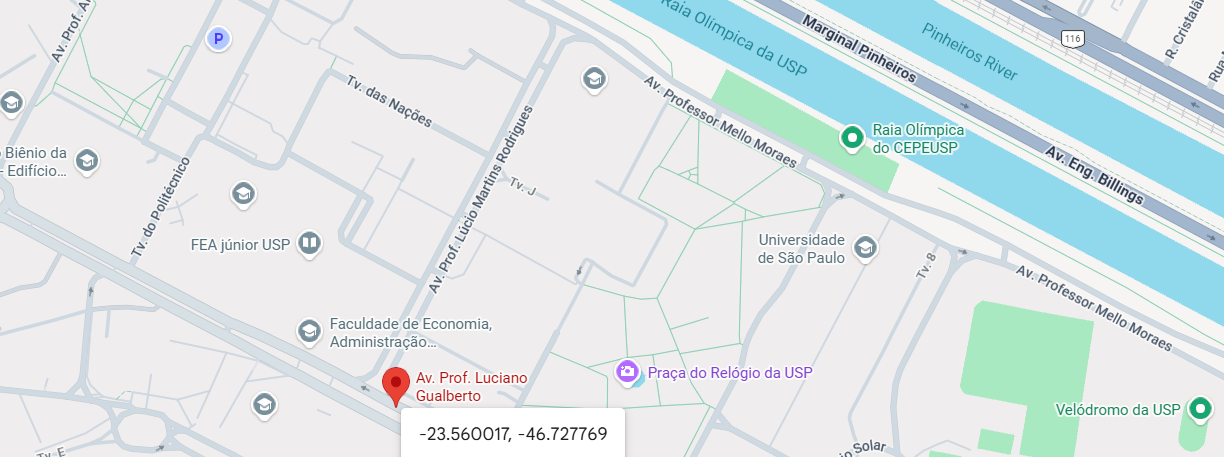
\includegraphics[width=0.94\linewidth]{images/Screenshot 2026-07-18 143636.png}
\end{center}

\emph{Figura 3 --- Consulta independente do endereço Avenida Professor
Luciano Gualberto, São Paulo, SP, no Google Maps. Fonte: captura de tela
do Google Maps realizada em 18 de julho de 2026.}

A Figura 4 mostra a consulta, no Google Maps, das coordenadas devolvidas
pelo motor; os dois pontos permanecem na Avenida Professor Luciano
Gualberto, na região da Universidade de São Paulo (USP).

\begin{center}
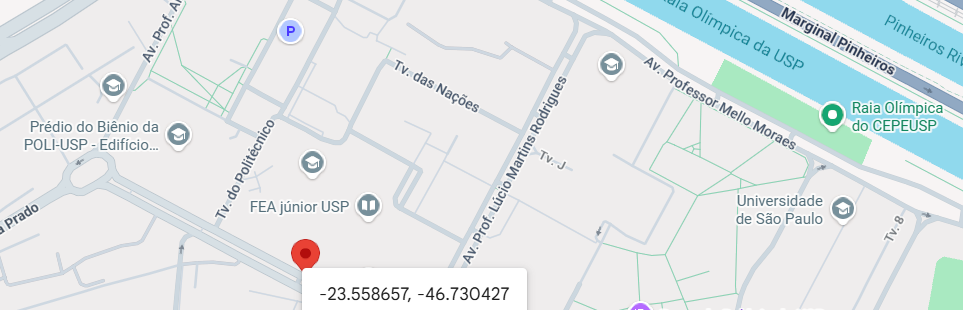
\includegraphics[width=0.94\linewidth]{images/Screenshot 2026-07-18 145249.png}
\end{center}

\emph{Figura 4 --- Consulta no Google Maps das coordenadas retornadas
pelo motor de geocodificação para a Avenida Professor Luciano Gualberto.
Fonte: captura de tela do Google Maps realizada em 18 de julho de 2026.}

Essa comparação confirma que as coordenadas apontam para a região
correta em escala de endereço. Ela não comprova precisão cadastral, como
a posição de um portão ou de um número específico do imóvel, mas é
suficiente para o propósito deste estudo.

\hypertarget{implementauxe7uxe3o-da-alternativa-rodoviuxe1ria}{%
\subsection{4.3 Implementação da alternativa
rodoviária}\label{implementauxe7uxe3o-da-alternativa-rodoviuxe1ria}}

\hypertarget{consulta-de-rota-rodoviuxe1ria}{%
\subsubsection{4.3.1 Consulta de rota
rodoviária}\label{consulta-de-rota-rodoviuxe1ria}}

Com as coordenadas da origem e do destino já definidas, o sistema envia
esse par primeiro ao OpenRouteService (ORS). Se o ORS não devolver uma
rota utilizável, envia o mesmo par ao LocationIQ. O provedor que
responder devolve a distância rodoviária e sua identificação, que ficam
associadas ao cenário.

No exemplo São Paulo--Rio Branco, após a geocodificação descrita na
Seção 4.2, o ORS recebeu as coordenadas de São Paulo (latitude
−23,550520°; longitude −46,633308°) e de Rio Branco (latitude
−9,989637°; longitude −67,822462°). A distância rodoviária devolvida foi
3.491,431~km.

\begin{center}
\resizebox{\linewidth}{!}{%
\begin{tikzpicture}
  \node[clnode] (mA) at (-5.50cm,2.00cm) {Origem: São Paulo, SP};
  \node[clnode] (mR) at (-5.50cm,0.00cm) {Geocodificação};
  \node[clnode] (mC) at (-5.50cm,-2.30cm) {Latitude: −23,550520°\\Longitude: −46,633308°};
  \node[clnode] (mB) at (-0.50cm,2.00cm) {Destino: Rio Branco, AC};
  \node[clnode] (mS) at (-0.50cm,0.00cm) {Geocodificação};
  \node[clnode] (mD) at (-0.50cm,-2.30cm) {Latitude: −9,989637°\\Longitude: −67,822462°};
  \node[clnode] (mT) at (4.20cm,-4.30cm) {Consulta de rota\\ORS/LocationIQ};
  \node[clnode] (mE) at (8.70cm,-4.30cm) {Distância rodoviária:\\3.491,431 km};
  \draw[clarrow] (mA) -- (mR);
  \draw[clarrow] (mB) -- (mS);
  \draw[clarrow] (mR) -- (mC);
  \draw[clarrow] (mS) -- (mD);
  \draw[clarrow] (mC) -- (mT);
  \draw[clarrow] (mD) -- (mT);
  \draw[clarrow] (mT) -- (mE);
\end{tikzpicture}%
}
\end{center}

\hypertarget{validauxe7uxe3o-da-distuxe2ncia-rodoviuxe1ria}{%
\paragraph{4.3.1.1 Validação da distância
rodoviária}\label{validauxe7uxe3o-da-distuxe2ncia-rodoviuxe1ria}}

A Figura 5 apresenta uma consulta independente no Google Maps para a
mesma ligação entre São Paulo e Rio Branco. A rota selecionada pelo
Google Maps tem 3.497~km, enquanto o motor do sistema retornou
3.491,431~km. A diferença é de 5,569~km, ou 0,16\% da distância exibida
no Google Maps.

\begin{center}
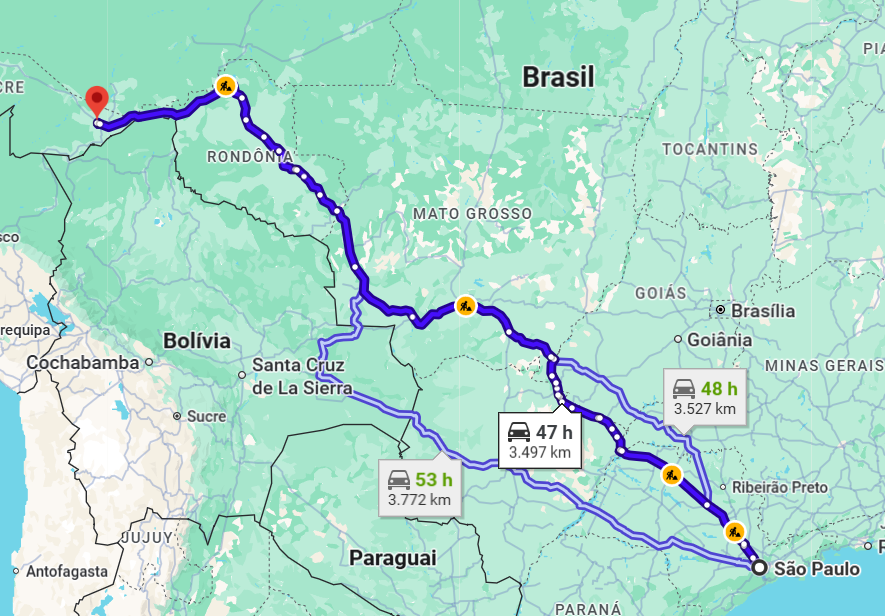
\includegraphics[width=0.94\linewidth]{images/Screenshot 2026-07-15 144749.png}
\end{center}

\emph{Figura 5 --- Consulta no Google Maps para São Paulo--Rio Branco:
rota selecionada de 3.497~km. Fonte: captura de tela do Google Maps
realizada em 15 de julho de 2026.}

Essa proximidade mostra que a distância usada no cálculo representa uma
rota pela malha rodoviária, e não a distância geográfica em linha reta
entre as cidades. Usar a distância em linha reta reduziria
artificialmente os quilômetros percorridos e poderia distorcer as
estimativas de consumo, custo e emissões.

\hypertarget{consulta-do-preuxe7o-do-diesel}{%
\subsubsection{4.3.2 Consulta do preço do
diesel}\label{consulta-do-preuxe7o-do-diesel}}

Para calcular o custo, a rotina Python busca os preços mais recentes de
Diesel S10. Ela baixa a planilha semanal de preços de revenda por estado
da Agência Nacional do Petróleo, Gás Natural e Biocombustíveis (ANP),
disponibilizada no
\href{https://www.gov.br/anp/pt-br/assuntos/precos-e-defesa-da-concorrencia/precos/precos-revenda-e-de-distribuicao-combustiveis/shlp/semanal/}{site
oficial da agência}.

Após confirmar que o XLSX baixado gerou uma tabela válida de preços por
Unidade da Federação (UF), a rotina também salva os dois arquivos no
Supabase Storage, o espaço de armazenamento de arquivos do projeto, para
garantir rastreabilidade e uma alternativa caso o site da ANP esteja
indisponível.

\textbf{Tabela 12 --- Recorte bruto da planilha semanal da ANP para
\texttt{OLEO\ DIESEL\ S10}.}

{\scriptsize
\renewcommand{\arraystretch}{0.78}
\begin{tabular}{@{}p{0.095\linewidth}p{0.095\linewidth}p{0.09\linewidth}p{0.14\linewidth}p{0.15\linewidth}p{0.13\linewidth}p{0.14\linewidth}@{}}
\toprule
\textbf{DATA\newline INICIAL} & \textbf{DATA\newline FINAL} & \textbf{REGIÃO} & \textbf{ESTADO} & \textbf{PRODUTO} & \textbf{UNIDADE\newline DE MEDIDA} & \raggedleft\textbf{PREÇO MÉDIO\newline REVENDA}\tabularnewline
\midrule
07-12-26 & 07-18-26 & SUDESTE & SAO PAULO & OLEO DIESEL S10 & R\$/l & \raggedleft 6.96\tabularnewline
07-12-26 & 07-18-26 & NORTE & ACRE & OLEO DIESEL S10 & R\$/l & \raggedleft 9.27\tabularnewline
07-12-26 & 07-18-26 & NORTE & AMAZONAS & OLEO DIESEL S10 & R\$/l & \raggedleft 7.25\tabularnewline
07-12-26 & 07-18-26 & NORDESTE & PERNAMBUCO & OLEO DIESEL S10 & R\$/l & \raggedleft 6.88\tabularnewline
\bottomrule
\end{tabular}
}

\emph{Fonte: planilha semanal de preços de revenda por estado da ANP,
aba \texttt{ESTADOS\ -\ DESDE\ 30.12.2012}, produto
\texttt{OLEO\ DIESEL\ S10}, período de 12 a 18 de julho de 2026. Valores
reproduzidos do arquivo \texttt{SEMANAL\_ESTADOS-DESDE\_2013.xlsx} usado
para conferir a rotina de leitura.}

\hypertarget{consumo-custo-e-emissuxf5es-rodoviuxe1rias}{%
\subsubsection{4.3.3 Consumo, custo e emissões
rodoviárias}\label{consumo-custo-e-emissuxf5es-rodoviuxe1rias}}

Com a distância disponível, o avaliador aplica as regras das Seções
3.2.1 a 3.2.3. Ele seleciona a configuração rodoviária representativa a
partir da massa da remessa, calcula os litros de diesel de cada perna e
converte esse consumo em custo e emissões.

Cada perna guarda, além do valor calculado, a distância, o tipo de
veículo, o preço de diesel, o fator de emissão e a origem desses
insumos. Dessa forma, o total rodoviário pode ser auditado sem
misturá-lo com as parcelas portuárias ou marítimas.

\hypertarget{resumo-do-pipeline-da-alternativa-direta}{%
\subsubsection{4.3.4 Resumo do pipeline da alternativa
direta}\label{resumo-do-pipeline-da-alternativa-direta}}

A alternativa direta é calculada de forma independente da alternativa
multimodal. O pipeline recebe origem, destino e carga; transforma os
locais em coordenadas; obtém a distância pela malha rodoviária;
seleciona o veículo representativo; estima o consumo de diesel; e, por
fim, converte esse consumo em custo modelado do combustível e emissões
operacionais. O resultado serve como referência para a comparação, sem
incluir portos ou navegação.

No exemplo São Paulo--Rio Branco, uma remessa de 14~t percorre
3.491,431~km. O sistema seleciona uma carreta de cinco eixos, com
eficiência de 2,3~km/L, e estima 1.518,014~L de Diesel S10. Com o preço
e o fator de emissão definidos nas Seções~3.2.2 e 3.2.3, o resultado é
R\$~12.318,68 de custo modelado do combustível e 4.068,28~kg~CO\textsubscript{2}e de
emissões operacionais TTW.

\begin{center}
\resizebox{\linewidth}{!}{%
\begin{tikzpicture}
  \node[clnode] (mA) at (0.00cm,0.00cm) {Carga, origem e destino\\14t de São Paulo até Rio Branco};
  \node[clnode] (mB) at (4.60cm,1.70cm) {Geocodificação};
  \node[clnode] (mC) at (9.20cm,1.70cm) {Distância rodoviária\\3.491,431 km};
  \node[clnode] (mD) at (4.60cm,-1.70cm) {Rendimento do veículo\\2,3 km/L de Diesel};
  \node[clnode] (mE) at (10.00cm,0.00cm) {Consumo de Diesel S10\\1.518,014 L};
  \node[clnode] (mP) at (15.00cm,3.00cm) {Preço do Diesel\\R\$ 8,115/L};
  \node[clnode] (mF) at (15.00cm,1.30cm) {Custo modelado do combustível\\R\$ 12.318,68};
  \node[clnode] (mM) at (15.00cm,-3.00cm) {Fator de emissão do Diesel\\2,68 kg CO\textsubscript{2}e/L};
  \node[clnode] (mG) at (15.00cm,-1.30cm) {Emissões TTW\\4.068,28 kg CO\textsubscript{2}e};
  \draw[clarrow] (mA) -- (mB);
  \draw[clarrow] (mA) -- (mD);
  \draw[clarrow] (mB) -- (mC);
  \draw[clarrow] (mC) -- (mE);
  \draw[clarrow] (mD) -- (mE);
  \draw[clarrow] (mE) -- (mF);
  \draw[clarrow] (mP) -- (mF);
  \draw[clarrow] (mE) -- (mG);
  \draw[clarrow] (mM) -- (mG);
\end{tikzpicture}%
}
\end{center}

\hypertarget{montagem-da-alternativa-multimodal}{%
\subsection{4.4 Montagem da alternativa
multimodal}\label{montagem-da-alternativa-multimodal}}

Após calcular a rota rodoviária direta, o sistema monta a alternativa
multimodal. Essa etapa reutiliza os veículos representativos do
transporte rodoviário, os endereços já geocodificados, os preços de
diesel por unidade federativa e a cotação do VLSFO.

\hypertarget{consulta-e-conversuxe3o-do-preuxe7o-do-vlsfo}{%
\subsubsection{4.4.1 Consulta e conversão do preço do
VLSFO}\label{consulta-e-conversuxe3o-do-preuxe7o-do-vlsfo}}

Antes de avaliar a alternativa multimodal, o pipeline busca a cotação
mais recente disponível do VLSFO (\emph{very low sulphur fuel oil}, óleo
combustível de baixíssimo teor de enxofre) na
\href{https://shipandbunker.com/prices/br-brazil}{Ship \& Bunker}. A
biblioteca Python \texttt{requests} acessa a página brasileira do
serviço e obtém o preço do VLSFO em dólares por tonelada métrica
(US\$/mt).

A cotação internacional precisa ser convertida antes de entrar no
cálculo de custo. A biblioteca Python
\href{https://pypi.org/project/CurrencyConverter/}{CurrencyConverter}
obtém a taxa USD/BRL a partir das referências do Banco Central Europeu
(BCE).

No exemplo São Paulo--Rio Branco, a conversão é:

\[
\begin{aligned}
P_{\mathrm{VLSFO}}^{\mathrm{R\$/mt}}
&= 741{,}50\ \mathrm{US\$/mt} \times 5{,}141345\ \mathrm{R\$/US\$} \\
&= 3.812{,}31\ \mathrm{R\$/mt}, \\[4pt]
P_{\mathrm{VLSFO}}^{\mathrm{R\$/kg}}
&= \frac{3.812{,}31\ \mathrm{R\$/mt}}{1.000\ \mathrm{kg/mt}} \\
&= 3{,}812\ \mathrm{R\$/kg}.
\end{aligned}
\]

Nas duas linhas, \(P_{\mathrm{VLSFO}}\) representa o preço do VLSFO e o
sobrescrito informa a unidade em que ele está expresso. Esse é o valor
entregue ao avaliador para calcular o custo do combustível marítimo. A
fonte, os valores e a regra de custo estão detalhados na Seção 3.3.6 e
na Tabela 8.

\hypertarget{matriz-maruxedtima}{%
\subsubsection{4.4.2 Matriz marítima}\label{matriz-maruxedtima}}

Antes de definir os portos de um novo cenário, o sistema prepara a
referência marítima com base em viagens de cabotagem que realmente
ocorreram. O produto dessa preparação é uma matriz marítima construída
com dados observados.

Quando a matriz não apresenta uma distância entre dois portos, a
implementação usa como fallback os dados de distância marítima publicados
pelo \href{https://www.geografos.com.br/}{Geógrafos}
\parencite{geografos2026}.

\hypertarget{dados-da-antaq}{%
\paragraph{4.4.2.1 Dados da ANTAQ}\label{dados-da-antaq}}

A rotina de atualização acessa o
\href{https://estatistica.antaq.gov.br/ea/sense/download.html}{Painel
Estatístico Aquaviário da ANTAQ}, portal oficial de download das tabelas
públicas. A biblioteca Python \texttt{requests} realiza as consultas e
baixa os arquivos em formato TXT. A biblioteca Python Beautiful Soup lê
a página e seus arquivos de apoio para localizar os endereços de
download disponibilizados pela ANTAQ. São obtidas as tabelas de Carga,
Atracação e Tempos de Atracação. Os campos de Carga e Atracação usados
na reconstrução estão detalhados na Seção 3.3.4.1, nas Tabelas 4 e 5.

A atualização também sincroniza os dados necessários e os artefatos
gerados para o Supabase Storage, o local de armazenamento de arquivos do
projeto. Dessa forma, os arquivos usados na reconstrução e a matriz
marítima permanecem disponíveis para reutilização e rastreabilidade, sem
depender do acesso imediato ao portal da ANTAQ.

\hypertarget{reconstruuxe7uxe3o-das-viagens-1}{%
\paragraph{4.4.2.2 Reconstrução das
viagens}\label{reconstruuxe7uxe3o-das-viagens-1}}

Para implementar a lógica apresentada na Seção 3.3.4.1.3, a função de
reconstrução reúne os registros de cabotagem conteinerizada e relaciona
cada movimentação de carga à escala correspondente. A tabela de
Atracação fornece o porto, a data e o número da Organização Marítima
Internacional (IMO) do navio; a tabela de Carga informa o que foi
embarcado e desembarcado.

Em seguida, as escalas do mesmo navio são reunidas em ordem cronológica.
A carga a bordo também é reconstruída em cada escala. O sistema calcula
o saldo entre o que embarcou e o que desembarcou do navio e aplica esse
saldo ao subtrecho seguinte. Quando o recorte de dados começa com o
navio já carregado, é calculada a carga inicial mínima necessária para
evitar valores negativos. A partir dessa reconstrução, em cada viagem, o
sistema identifica os pares de portos em que o navio atracou primeiro na
origem e, posteriormente, no destino. A parte da viagem entre essas duas
escalas forma um recorte completo, direto ou com escalas intermediárias.
Por exemplo, Santos--Suape--Pecém--Manaus contribui para Santos--Manaus
com seus três subtrechos; Manaus--Suape--Santos não contribui, pois está
no sentido contrário.

O resultado da reconstrução também é gravado em tabelas criadas no banco
de dados do projeto no Supabase PostgreSQL, o que permite consultar as
viagens já reconstruídas sem repetir o processamento dos arquivos
brutos:

\begin{itemize}
\tightlist
\item
  A tabela \texttt{antaq\_voyages} registra cada viagem reconstruída;
\item
  A tabela \texttt{antaq\_voyage\_stops} armazena suas paradas em ordem;
\item
  A tabela\texttt{antaq\_voyage\_stop\_calls} preserva as escalas que
  formaram cada parada.
\end{itemize}

\hypertarget{dados-da-eu-mrv}{%
\paragraph{4.4.2.3 Dados da EU MRV}\label{dados-da-eu-mrv}}

Os arquivos anuais da base europeia de Monitoramento, Reporte e
Verificação da União Europeia (EU MRV) são obtidos no
\href{https://mrv.emsa.europa.eu/}{THETIS-MRV, da Agência Europeia de
Segurança Marítima} e armazenados no Supabase Storage. Os campos e o
exemplo de correspondência por IMO estão apresentados na Seção 3.3.4.2 e
na Tabela 6.

\hypertarget{cuxe1lculo-do-trabalho-de-transporte}{%
\paragraph{4.4.2.4 Cálculo do trabalho de
transporte}\label{cuxe1lculo-do-trabalho-de-transporte}}

Como explicado na Seção 3.3.4.2, o sistema procura primeiro o IMO do
navio observado na ANTAQ. Se não houver indicador individual utilizável,
ou se ele for classificado como atípico, é aplicada uma referência
robusta de navios da mesma classe ou, se necessário, do mesmo tipo. A
carga a bordo, a distância e a intensidade permitem calcular o trabalho
de transporte e o consumo estimado de cada viagem.

\hypertarget{compilauxe7uxe3o-na-estrutura-matricial}{%
\paragraph{4.4.2.5 Compilação na estrutura
matricial}\label{compilauxe7uxe3o-na-estrutura-matricial}}

Os resultados são reunidos na estrutura \texttt{SeaMatrix}. Para cada
par ordenado de portos, ela mantém a distância representativa dos
recortes completos após a verificação de P95, ponderada pela carga média
a bordo, e a intensidade, ponderada pelo trabalho de transporte de todos
os recortes elegíveis. Também registra a quantidade de recortes, o limite
P95 quando aplicável e a procedência dos dados. A matriz é direcional:
Santos → Manaus e Manaus → Santos são consultas diferentes, pois reúnem
viagens, cargas e distâncias observadas diferentes. A \texttt{SeaMatrix}
também é salva no Supabase Storage como o arquivo JSON
\texttt{data/sea\_matrix.json}.

\begin{center}
\resizebox{\linewidth}{!}{%
\begin{tikzpicture}
  \node[clnode] (mA) at (0.00cm,1.70cm) {Carga e Atracação\\ANTAQ};
  \node[clnode] (mB) at (5.10cm,1.70cm) {Reconstrução das viagens\\e da carga a bordo};
  \node[clnode] (mC) at (10.20cm,1.70cm) {Recortes completos\\entre portos ordenados};
  \node[clnode] (mD) at (0.00cm,-1.70cm) {EU MRV\\intensidade por IMO};
  \node[clnode] (mE) at (5.10cm,-1.70cm) {Intensidade individual\\ou referência robusta};
  \node[clnode] (mT) at (10.20cm,-1.70cm) {Trabalho de transporte\\e consumo por recorte};
  \node[clnode] (mF) at (15.30cm,-1.70cm) {SeaMatrix\\distância, intensidade\\e cobertura};
  \draw[clarrow] (mA) -- (mB);
  \draw[clarrow] (mB) -- (mC);
  \draw[clarrow] (mD) -- (mE);
  \draw[clarrow] (mC) -- (mT);
  \draw[clarrow] (mE) -- (mT);
  \draw[clarrow] (mT) -- (mF);
\end{tikzpicture}%
}
\end{center}

As Tabelas 13 e 14 mostram parte da matriz marítima preparada com dados
reais. As linhas indicam o porto de origem e, as colunas, o porto de
destino.

A Tabela 13 apresenta a distância representativa de cada sentido. Quando
há 20 ou mais recortes, as distâncias acima do P95 são retiradas antes da
média ponderada pela carga média a bordo, conforme explicado na
Seção~3.3.4.4. Nota-se que a distância de ida pode ser diferente da
distância de volta, uma vez que cada sentido reúne seu próprio conjunto
de viagens, cargas e distâncias observadas. As duas tabelas incluem
recortes diretos e recortes com escalas intermediárias. O travessão
indica que origem e destino são o mesmo porto, situação que não forma
uma perna marítima.

\textbf{Tabela 13 --- Distância marítima representativa após a triagem
P95, ponderada pela carga média a bordo, na matriz marítima (km).}

\begin{longtable}[]{@{}lrrrrr@{}}
\toprule
Origem / destino & Santos & Salvador & Suape & Pecém &
Manaus\tabularnewline
\midrule
\endhead
Santos & --- & 2.516,136 & 2.912,073 & 3.578,767 &
6.094,975\tabularnewline
Salvador & 2.867,589 & --- & 4.122,437 & 3.475,834 &
3.819,166\tabularnewline
Suape & 3.800,410 & 2.801,434 & --- & 940,458 &
3.214,997\tabularnewline
Pecém & 4.103,118 & 2.437,283 & 5.301,235 & --- &
2.195,720\tabularnewline
Manaus & 5.867,445 & 6.585,233 & 5.560,801 & 5.768,673 &
---\tabularnewline
\bottomrule
\end{longtable}

\emph{Fonte: elaboração própria a partir da matriz marítima direcional
preparada com viagens de cabotagem observadas pela ANTAQ, atualizada em
19 de julho de 2026.}

\Needspace{14\baselineskip}
A Tabela 14 apresenta a intensidade média, ponderada pelo trabalho de
transporte.

\textbf{Tabela 14 --- Intensidade média da ligação marítima, ponderada
pelo trabalho de transporte {[}g/(t·nm){]}.}

\begin{longtable}[]{@{}lrrrrr@{}}
\toprule
Origem / destino & Santos & Salvador & Suape & Pecém &
Manaus\tabularnewline
\midrule
\endhead
Santos & --- & 9,605744 & 8,729368 & 9,745651 & 9,009824\tabularnewline
Salvador & 9,338150 & --- & 8,558943 & 10,183560 &
9,322050\tabularnewline
Suape & 9,292748 & 9,984933 & --- & 9,551157 & 9,034616\tabularnewline
Pecém & 9,643543 & 9,716983 & 8,681143 & --- & 9,092814\tabularnewline
Manaus & 9,098669 & 9,322050 & 9,178646 & 9,055626 & ---\tabularnewline
\bottomrule
\end{longtable}

\emph{Fonte: elaboração própria a partir de viagens de cabotagem
observadas pela ANTAQ e das intensidades do EU MRV, consolidadas na
matriz marítima direcional atualizada em 19 de julho de 2026.}

O trecho abaixo representa, de forma simplificada, como a matriz pode
ser consultada. O porto de origem contém os portos de destino e, para
cada ligação, ficam disponíveis a distância representativa e a
intensidade média. Foram exibidos apenas três destinos de Santos para
manter a visualização curta; o arquivo real também guarda a procedência
e os indicadores de cobertura apresentados nas seções anteriores.

\textbf{Bloco de código 1 --- Representação simplificada do arquivo
\texttt{sea\_matrix.json}.}

\begin{Shaded}
\begin{Highlighting}[]
\FunctionTok{\{}
    \DataTypeTok{"Porto de Santos"}\FunctionTok{:} \FunctionTok{\{}
        \DataTypeTok{"Porto de Salvador"}\FunctionTok{:} \FunctionTok{\{}
            \DataTypeTok{"distancia_km"}\FunctionTok{:} \FloatTok{2516.136}\FunctionTok{,}
            \DataTypeTok{"intensidade_g_por_t_nm"}\FunctionTok{:} \FloatTok{9.605744}\FunctionTok{,}
            \ErrorTok{...}
        \FunctionTok{\},}
    \DataTypeTok{"Porto de Suape"}\FunctionTok{:} \FunctionTok{\{}
        \DataTypeTok{"distancia_km"}\FunctionTok{:} \FloatTok{2912.073}\FunctionTok{,}
        \DataTypeTok{"intensidade_g_por_t_nm"}\FunctionTok{:} \FloatTok{8.729368}\FunctionTok{,}
        \ErrorTok{...}
    \FunctionTok{\},}
    \DataTypeTok{"Porto de Manaus"}\FunctionTok{:} \FunctionTok{\{}
      \DataTypeTok{"distancia_km"}\FunctionTok{:} \FloatTok{6094.975}\FunctionTok{,}
      \DataTypeTok{"intensidade_g_por_t_nm"}\FunctionTok{:} \FloatTok{9.009824}\FunctionTok{,}
      \ErrorTok{...}
    \FunctionTok{\},}
    \ErrorTok{...}
  \FunctionTok{\},}
\ErrorTok{...}
\FunctionTok{\}}
\end{Highlighting}
\end{Shaded}

\hypertarget{escolha-dos-portos-e-acessos-rodoviuxe1rios}{%
\subsubsection{4.4.3 Escolha dos portos e acessos
rodoviários}\label{escolha-dos-portos-e-acessos-rodoviuxe1rios}}

\hypertarget{escolha-dos-portos-1}{%
\paragraph{4.4.3.1 Escolha dos portos}\label{escolha-dos-portos-1}}

A definição dos portos de embarque e desembarque começa pela função
\texttt{find\_nearest\_port}. Ela usa a distância de Haversine, um
cálculo geométrico realizado a partir das latitudes e longitudes, que
estima a menor distância sobre a superfície da Terra entre dois pontos.
Esse cálculo é rápido, executado localmente e não representa uma rota
por estrada. A função mede a distância entre o ponto de origem ou
destino e cada porto disponível e seleciona o porto com a menor
distância. O pipeline executa a função uma vez para as coordenadas da
origem, definindo o porto de embarque, e outra vez para as coordenadas
do destino, definindo o porto de desembarque.

A distância de Haversine, porém, é usada apenas nessa escolha inicial.
Ela não entra nos cálculos de consumo, custo ou emissões.

\hypertarget{acessos-rodoviuxe1rios-first-mile-e-last-mile-1}{%
\paragraph{\texorpdfstring{4.4.3.2 Acessos rodoviários: \emph{first
mile} e \emph{last
mile}}{4.4.3.2 Acessos rodoviários: first mile e last mile}}\label{acessos-rodoviuxe1rios-first-mile-e-last-mile-1}}

Após escolher os dois portos e suas respectivas coordenadas, o sistema
calcula a distância real dos dois acessos rodoviários --- origem → porto
de embarque e porto de desembarque → destino --- pelo mesmo procedimento
exposto na Seção 4.3.1.

Essa sequência reduz consultas desnecessárias aos provedores de rota. Em
vez de solicitar uma rota rodoviária para cada porto candidato de uma
coordenada, o sistema faz uma única consulta para o acesso do porto já
selecionado. Assim, a distância usada no cálculo continua sendo
rodoviária, enquanto a distância de Haversine é usada apenas como um
filtro rápido para definir qual porto consultar.

\hypertarget{resultado-consolidado-do-exemplo-suxe3o-paulorio-branco}{%
\paragraph{4.4.3.3 Resultado consolidado do exemplo São Paulo--Rio
Branco}\label{resultado-consolidado-do-exemplo-suxe3o-paulorio-branco}}

No exemplo São Paulo--Rio Branco, a seleção geográfica indicou o Porto
de Santos para o embarque e o Porto de Manaus para o desembarque. A
Tabela 15 compara a distância de Haversine usada na seleção com a
distância rodoviária calculada após a escolha de cada porto.

\textbf{Tabela 15 --- Distâncias de seleção e de acesso rodoviário no
exemplo São Paulo--Rio Branco.}

\begin{longtable}[]{@{}lllrr@{}}
\toprule
\begin{minipage}[b]{0.17\columnwidth}\raggedright
Acesso\strut
\end{minipage} & \begin{minipage}[b]{0.17\columnwidth}\raggedright
Ponto geocodificado\strut
\end{minipage} & \begin{minipage}[b]{0.17\columnwidth}\raggedright
Referência do porto\strut
\end{minipage} & \begin{minipage}[b]{0.17\columnwidth}\raggedleft
Haversine: seleção\strut
\end{minipage} & \begin{minipage}[b]{0.17\columnwidth}\raggedleft
Distância rodoviária: cálculo\strut
\end{minipage}\tabularnewline
\midrule
\endhead
\begin{minipage}[t]{0.17\columnwidth}\raggedright
\emph{First mile}:\newline{}São Paulo → Porto de Santos\strut
\end{minipage} & \begin{minipage}[t]{0.17\columnwidth}\raggedright
São Paulo (origem):\newline{}{[}−23,550520°; −46,633308°{]}\strut
\end{minipage} & \begin{minipage}[t]{0.17\columnwidth}\raggedright
Porto de Santos (embarque):\newline{}{[}−23,987012°;
−46,293383°{]}\strut
\end{minipage} & \begin{minipage}[t]{0.17\columnwidth}\raggedleft
59,601~km\strut
\end{minipage} & \begin{minipage}[t]{0.17\columnwidth}\raggedleft
86,170~km\strut
\end{minipage}\tabularnewline
\begin{minipage}[t]{0.17\columnwidth}\raggedright
\emph{Last mile}:\newline{}Porto de Manaus → Rio Branco\strut
\end{minipage} & \begin{minipage}[t]{0.17\columnwidth}\raggedright
Rio Branco (destino):\newline{}{[}−9,989637°; −67,822462°{]}\strut
\end{minipage} & \begin{minipage}[t]{0.17\columnwidth}\raggedright
Porto de Manaus (desembarque):\newline{}{[}−3,156700°;
−60,007900°{]}\strut
\end{minipage} & \begin{minipage}[t]{0.17\columnwidth}\raggedleft
1.149,569~km\strut
\end{minipage} & \begin{minipage}[t]{0.17\columnwidth}\raggedleft
1.403,691~km\strut
\end{minipage}\tabularnewline
\bottomrule
\end{longtable}

\emph{Fonte: elaboração própria com a base de portos do sistema e as
rotas rodoviárias obtidas no cenário.}

A diferença entre as duas colunas é esperada: Haversine mede a separação
geométrica entre os pontos, enquanto a distância rodoviária acompanha o
caminho percorrido pela malha viária. Apenas a última é usada nos
cálculos da alternativa multimodal.

\hypertarget{operauxe7uxf5es-portuuxe1rias-1}{%
\subsubsection{4.4.4 Operações
portuárias}\label{operauxe7uxf5es-portuuxe1rias-1}}

A rotina de operações portuárias recebe a carga, os dois portos e o
número de escalas para realizar o procedimento descrito na Seção 3.3.3.
O resultado da execução foi 4,820~L de diesel para as operações
quantificadas, equivalentes a R\$~34,25 e 12,92~kg~CO\textsubscript{2}e.

\hypertarget{consulta-da-ligauxe7uxe3o-maruxedtima}{%
\subsection{4.5 Consulta da ligação
marítima}\label{consulta-da-ligauxe7uxe3o-maruxedtima}}

Com os portos de embarque e desembarque já definidos, o avaliador
consulta a matriz preparada na Seção 4.4.2. Nessa etapa, ele não escolhe
um novo corredor nem reconstrói as viagens históricas: apenas recupera
os valores representativos do par de portos selecionado e os aplica à
carga do cenário.

\hypertarget{consulta-da-ligauxe7uxe3o-maruxedtima-no-cenuxe1rio}{%
\subsubsection{4.5.1 Consulta da ligação marítima no
cenário}\label{consulta-da-ligauxe7uxe3o-maruxedtima-no-cenuxe1rio}}

No exemplo São Paulo--Rio Branco, a escolha dos portos leva à consulta
Santos--Manaus na \texttt{SeaMatrix}. A Tabela~16 mostra o que a matriz
devolve para esse par. Um recorte é a parte de uma viagem observada
compreendida entre os dois portos da ligação; ele pode ser direto ou
conter escalas intermediárias.

\textbf{Tabela 16 --- Informações devolvidas pela matriz marítima para a
ligação Santos--Manaus.}

\begin{longtable}[]{@{}lll@{}}
\toprule
\begin{minipage}[b]{0.30\columnwidth}\raggedright
Informação\strut
\end{minipage} & \begin{minipage}[b]{0.30\columnwidth}\raggedright
Valor retornado na execução\strut
\end{minipage} & \begin{minipage}[b]{0.30\columnwidth}\raggedright
Como deve ser lido\strut
\end{minipage}\tabularnewline
\midrule
\endhead
\begin{minipage}[t]{0.30\columnwidth}\raggedright
Cobertura observada\strut
\end{minipage} & \begin{minipage}[t]{0.30\columnwidth}\raggedright
89 recortes em 22 corredores\strut
\end{minipage} & \begin{minipage}[t]{0.30\columnwidth}\raggedright
Todas as viagens em que Santos aparece antes de Manaus são consideradas
no mesmo sentido\strut
\end{minipage}\tabularnewline
\begin{minipage}[t]{0.30\columnwidth}\raggedright
Forma dos recortes\strut
\end{minipage} & \begin{minipage}[t]{0.30\columnwidth}\raggedright
1 direto e 88 com escalas intermediárias\strut
\end{minipage} & \begin{minipage}[t]{0.30\columnwidth}\raggedright
Não há corredor obrigatório nem seleção do percurso mais curto\strut
\end{minipage}\tabularnewline
\begin{minipage}[t]{0.30\columnwidth}\raggedright
Amostra da distância\strut
\end{minipage} & \begin{minipage}[t]{0.30\columnwidth}\raggedright
87 recortes em 20 corredores; P95 de 6.975,000~km\strut
\end{minipage} & \begin{minipage}[t]{0.30\columnwidth}\raggedright
Os 2 recortes acima do P95 permanecem auditáveis, mas não entram na
média de distância\strut
\end{minipage}\tabularnewline
\begin{minipage}[t]{0.30\columnwidth}\raggedright
Distância marítima\strut
\end{minipage} & \begin{minipage}[t]{0.30\columnwidth}\raggedright
6.094,975~km, ou 3.291,023~nm\strut
\end{minipage} & \begin{minipage}[t]{0.30\columnwidth}\raggedright
Média da distância total, ponderada pela carga média a bordo dos 87
recortes até o P95\strut
\end{minipage}\tabularnewline
\begin{minipage}[t]{0.30\columnwidth}\raggedright
Intensidade marítima\strut
\end{minipage} & \begin{minipage}[t]{0.30\columnwidth}\raggedright
9,009824~g/(t·nm)\strut
\end{minipage} & \begin{minipage}[t]{0.30\columnwidth}\raggedright
Média ponderada pelo trabalho de transporte dos 89 recortes\strut
\end{minipage}\tabularnewline
\begin{minipage}[t]{0.30\columnwidth}\raggedright
Origem das intensidades\strut
\end{minipage} & \begin{minipage}[t]{0.30\columnwidth}\raggedright
19 por IMO; 49 por tipo sem IMO utilizável; 21 por tipo após tratamento
de valor atípico\strut
\end{minipage} & \begin{minipage}[t]{0.30\columnwidth}\raggedright
A fonte permanece identificada para cada recorte\strut
\end{minipage}\tabularnewline
\begin{minipage}[t]{0.30\columnwidth}\raggedright
Aviso de distância\strut
\end{minipage} & \begin{minipage}[t]{0.30\columnwidth}\raggedright
1 subtrecho aproximado por haversine entre 391 subtrechos\strut
\end{minipage} & \begin{minipage}[t]{0.30\columnwidth}\raggedright
A aproximação permanece identificada na amostra de distância usada no
cenário\strut
\end{minipage}\tabularnewline
\bottomrule
\end{longtable}

\hypertarget{resultado-final-do-cenuxe1rio}{%
\subsection{4.6 Resultado final do
cenário}\label{resultado-final-do-cenuxe1rio}}

Após executar as etapas descritas nas seções anteriores, o pipeline
reúne os totais das duas alternativas para a mesma remessa. A Tabela 17
apresenta o resultado final do exemplo São Paulo--Rio Branco, com 14~t
de carga.

\textbf{Tabela 17 --- Resultado final do cenário São Paulo--Rio Branco.}

\begin{longtable}[]{@{}lrrl@{}}
\toprule
\begin{minipage}[b]{0.22\columnwidth}\raggedright
Indicador\strut
\end{minipage} & \begin{minipage}[b]{0.22\columnwidth}\raggedleft
Rodovia direta\strut
\end{minipage} & \begin{minipage}[b]{0.22\columnwidth}\raggedleft
Alternativa multimodal\strut
\end{minipage} & \begin{minipage}[b]{0.22\columnwidth}\raggedright
Diferença da alternativa multimodal\strut
\end{minipage}\tabularnewline
\midrule
\endhead
\begin{minipage}[t]{0.22\columnwidth}\raggedright
Distância percorrida\strut
\end{minipage} & \begin{minipage}[t]{0.22\columnwidth}\raggedleft
3.491,431~km\strut
\end{minipage} & \begin{minipage}[t]{0.22\columnwidth}\raggedleft
7.584,836~km\strut
\end{minipage} & \begin{minipage}[t]{0.22\columnwidth}\raggedright
4.093,405~km a mais (117,24\%)\strut
\end{minipage}\tabularnewline
\begin{minipage}[t]{0.22\columnwidth}\raggedright
Custo modelado do combustível\strut
\end{minipage} & \begin{minipage}[t]{0.22\columnwidth}\raggedleft
R\$~12.318,68\strut
\end{minipage} & \begin{minipage}[t]{0.22\columnwidth}\raggedleft
R\$~6.918,66\strut
\end{minipage} & \begin{minipage}[t]{0.22\columnwidth}\raggedright
R\$~5.400,02 a menos (43,84\%)\strut
\end{minipage}\tabularnewline
\begin{minipage}[t]{0.22\columnwidth}\raggedright
Emissões operacionais TTW\strut
\end{minipage} & \begin{minipage}[t]{0.22\columnwidth}\raggedleft
4.068,28~kg~CO\textsubscript{2}e\strut
\end{minipage} & \begin{minipage}[t]{0.22\columnwidth}\raggedleft
3.041,62~kg~CO\textsubscript{2}e\strut
\end{minipage} & \begin{minipage}[t]{0.22\columnwidth}\raggedright
1.026,66~kg~CO\textsubscript{2}e a menos (25,24\%)\strut
\end{minipage}\tabularnewline
\bottomrule
\end{longtable}

\hypertarget{rastreabilidade-auditoria-e-versionamento}{%
\subsection{4.7 Rastreabilidade, auditoria e
versionamento}\label{rastreabilidade-auditoria-e-versionamento}}

O resultado não guarda apenas os totais de custo e emissão. A cada
execução, o pipeline registra os dados que formaram a rota, as fontes
utilizadas e os avisos que afetam a leitura do resultado. A Tabela~18
exemplifica esse registro no cenário São Paulo--Rio Branco.

\textbf{Tabela 18 --- Informações de rastreabilidade registradas no
exemplo São Paulo--Rio Branco.}

\begin{longtable}[]{@{}lll@{}}
\toprule
\begin{minipage}[b]{0.30\columnwidth}\raggedright
Informação registrada\strut
\end{minipage} & \begin{minipage}[b]{0.30\columnwidth}\raggedright
Exemplo no cenário\strut
\end{minipage} & \begin{minipage}[b]{0.30\columnwidth}\raggedright
Finalidade\strut
\end{minipage}\tabularnewline
\midrule
\endhead
\begin{minipage}[t]{0.30\columnwidth}\raggedright
Rota rodoviária direta\strut
\end{minipage} & \begin{minipage}[t]{0.30\columnwidth}\raggedright
3.491,431~km; resultado originalmente obtido do ORS e reutilizado na
execução\strut
\end{minipage} & \begin{minipage}[t]{0.30\columnwidth}\raggedright
Permite conferir a distância usada na alternativa direta\strut
\end{minipage}\tabularnewline
\begin{minipage}[t]{0.30\columnwidth}\raggedright
Portos selecionados\strut
\end{minipage} & \begin{minipage}[t]{0.30\columnwidth}\raggedright
Santos (SP) e Manaus (AM)\strut
\end{minipage} & \begin{minipage}[t]{0.30\columnwidth}\raggedright
Mostra onde começam e terminam os acessos marítimos e rodoviários\strut
\end{minipage}\tabularnewline
\begin{minipage}[t]{0.30\columnwidth}\raggedright
Ligação marítima\strut
\end{minipage} & \begin{minipage}[t]{0.30\columnwidth}\raggedright
89 viagens completas em 22 corredores; 87 recortes até o P95 para a
distância\strut
\end{minipage} & \begin{minipage}[t]{0.30\columnwidth}\raggedright
Identifica a base da intensidade e da distância marítimas\strut
\end{minipage}\tabularnewline
\begin{minipage}[t]{0.30\columnwidth}\raggedright
Intensidade marítima\strut
\end{minipage} & \begin{minipage}[t]{0.30\columnwidth}\raggedright
9,009824~g/(t·nm); fontes por IMO e por tipo identificadas\strut
\end{minipage} & \begin{minipage}[t]{0.30\columnwidth}\raggedright
Diferencia medição individual de estimativa de grupo\strut
\end{minipage}\tabularnewline
\begin{minipage}[t]{0.30\columnwidth}\raggedright
Operações portuárias\strut
\end{minipage} & \begin{minipage}[t]{0.30\columnwidth}\raggedright
RTG e caminhão interno do terminal\strut
\end{minipage} & \begin{minipage}[t]{0.30\columnwidth}\raggedright
Identifica os equipamentos considerados no cálculo\strut
\end{minipage}\tabularnewline
\begin{minipage}[t]{0.30\columnwidth}\raggedright
Preços de combustível\strut
\end{minipage} & \begin{minipage}[t]{0.30\columnwidth}\raggedright
Diesel S10 da ANP e VLSFO da Ship \& Bunker, com data e valor
usados\strut
\end{minipage} & \begin{minipage}[t]{0.30\columnwidth}\raggedright
Permite atualizar ou repetir o componente de custo\strut
\end{minipage}\tabularnewline
\begin{minipage}[t]{0.30\columnwidth}\raggedright
Avisos de qualidade\strut
\end{minipage} & \begin{minipage}[t]{0.30\columnwidth}\raggedright
Um subtrecho marítimo aproximado por haversine\strut
\end{minipage} & \begin{minipage}[t]{0.30\columnwidth}\raggedright
Sinaliza a aproximação sem ocultá-la no total\strut
\end{minipage}\tabularnewline
\bottomrule
\end{longtable}

\emph{Esses são os mesmos dados consolidados na Tabela 9 da Sessão
3.3.7}

\hypertarget{versionamento-e-reproduuxe7uxe3o-do-cuxe1lculo}{%
\subsubsection{4.7.1 Versionamento e reprodução do
cálculo}\label{versionamento-e-reproduuxe7uxe3o-do-cuxe1lculo}}

O versionamento é etapa fundamental do desenvolvimento de sistemas. Git
é uma ferramenta que registra o histórico das alterações feitas nos
arquivos de um projeto. O GitHub é a plataforma on-line em que esse
histórico é armazenado e pode ser consultado. O código e os documentos
do CabotageLens estão disponíveis
\href{https://github.com/pennylanesccp/cabotage-lens}{no repositório
público do GitHub}. Esse registro permite identificar quais regras e
arquivos foram usados em cada versão do estudo, comparar alterações e
apoiar a rastreabilidade e a auditoria dos resultados.

\hypertarget{aplicauxe7uxe3o-web}{%
\subsection{4.8 Aplicação web}\label{aplicauxe7uxe3o-web}}

Para disponibilizar o cálculo sem exigir instalação local, o
CabotageLens é hospedado gratuitamente no Streamlit Community Cloud. A
aplicação reúne duas interfaces diretamente relacionadas às análises
deste trabalho: a página Router, voltada à comparação de uma origem com
um destino, e a página Mapa de calor, destinada à visualização de
resultados para vários destinos. As subseções seguintes apresentam essas
duas interfaces.

\hypertarget{puxe1gina-router}{%
\subsubsection{4.8.1 Página Router}\label{puxe1gina-router}}

A página Router executa a comparação para a origem, o destino e a carga
informados no cenário. A Figura 6 mostra os campos da barra lateral
usados nessa definição. No exemplo, a análise parte da Avenida Professor
Luciano Gualberto, em São Paulo, segue para Manaus e considera uma carga
de 14 t.

\begin{center}
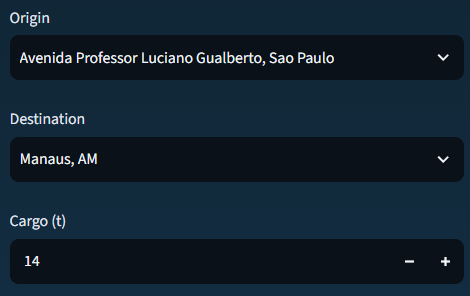
\includegraphics[width=0.94\linewidth]{images/router-scenario.png}
\end{center}

\emph{Figura 6 --- Campos de definição do cenário na página Router.
Fonte: elaboração própria.}

Após a execução, a página apresenta as alternativas calculadas em um
mapa, como ilustra a Figura 7. As linhas traçadas servem apenas para
representar visualmente as distâncias e a ligação entre os pontos; elas
não correspondem às rotas rodoviárias ou marítimas efetivamente
utilizadas nos cálculos.

\begin{center}
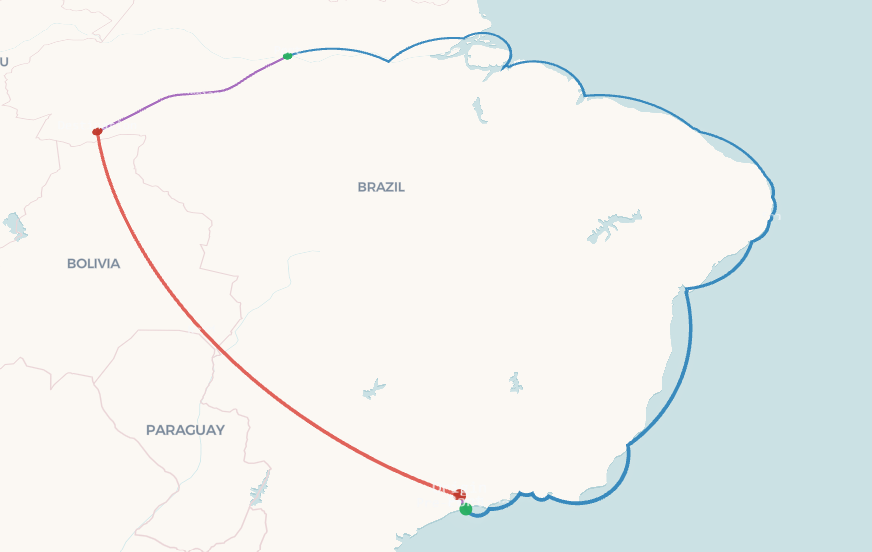
\includegraphics[width=0.94\linewidth]{images/router-map.png}
\end{center}

\emph{Figura 7 --- Representação visual das alternativas calculadas na
página Router. Fonte: elaboração própria.}

Os resultados detalhados, os avisos, os logs e os demais registros
gerados durante a execução podem ser consultados na própria página.
Assim, o mapa facilita a leitura espacial do cenário, enquanto a
conferência do cálculo é feita pelos dados e registros apresentados pelo
sistema.

\hypertarget{puxe1gina-mapa-de-calor}{%
\subsubsection{4.8.2 Página Mapa de
calor}\label{puxe1gina-mapa-de-calor}}

O Mapa de calor amplia a comparação realizada na página Router. Em vez
de avaliar apenas uma ligação entre origem e destino, o usuário informa
uma origem e a massa da carga, e o sistema compara esse cenário com 608
municípios brasileiros de população superior a 50 mil habitantes. Para
cada município, são calculadas as mesmas duas alternativas descritas na
Seção 3: a rodovia direta e a cadeia rodoviária--cabotagem--rodoviária.
A Figura 8 mostra os campos usados para definir o cenário. No exemplo, a
análise parte da Avenida Professor Luciano Gualberto, em São Paulo, e
considera uma carga de 14 t.

\begin{center}
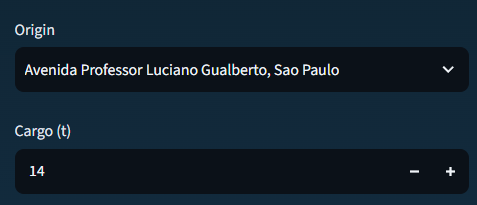
\includegraphics[width=0.94\linewidth]{images/heatmap-scenario.png}
\end{center}

\emph{Figura 8 --- Campos de definição do cenário na página Mapa de
calor. Fonte: elaboração própria.}

O resultado permite visualizar, em diferentes partes do país, onde a
alternativa multimodal com cabotagem apresenta vantagem em relação à
rodovia direta. O usuário pode escolher se o mapa representa custo
modelado do combustível ou emissões operacionais. Em cada destino, um
valor positivo indica que a alternativa multimodal teve menor custo ou
menor emissão; um valor negativo indica que a rodovia direta apresentou
o menor resultado para o indicador selecionado.

As cores e a altura da superfície facilitam a leitura espacial dessas
diferenças. Os resultados são calculados para os municípios do conjunto
de destinos; as áreas entre eles são uma interpolação visual para tornar
o padrão mais legível no mapa. Portanto, cada área colorida não
representa uma nova rota calculada, mas a visualização dos resultados
obtidos para os destinos próximos. A Figura 9 ilustra essa representação
para o cenário informado.

\begin{center}
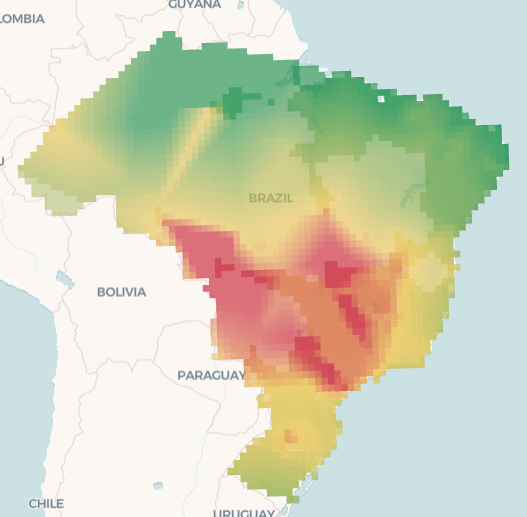
\includegraphics[width=0.94\linewidth]{images/heatmap-map.png}
\end{center}

\emph{Figura 9 --- Representação espacial dos resultados calculados na
página Mapa de calor. Fonte: elaboração própria.}

\hypertarget{comparauxe7uxf5es-com-ferramentas-externas}{%
\section{5. Comparações com ferramentas
externas}\label{comparauxe7uxf5es-com-ferramentas-externas}}

As ferramentas externas permitem confrontar o resultado do CabotageLens
com estimativas já disponíveis ao público. Em cada caso, são apresentadas as distâncias, as emissões ou os valores
de custo disponíveis na respectiva ferramenta. Quando a rota, o porto ou outro parâmetro
difere, a diferença permanece explícita; os resultados não são ajustados
para produzir uma equivalência artificial.

\hypertarget{calculadora-de-emissuxf5es-da-alianuxe7a}{%
\subsection{\texorpdfstring{5.1
\href{https://www.alianca.com.br/calculadora-de-co2}{Calculadora de
emissões da
Aliança}}{5.1 Calculadora de emissões da Aliança}}\label{calculadora-de-emissuxf5es-da-alianuxe7a}}

Na calculadora da Aliança \parencite{alianca2026}, o cenário informado foi São
Paulo--Abaetetuba, com um contêiner seco de 40 pés e 20 t de carga. O
mesmo cenário foi executado no CabotageLens com 20 t e 2 TEU,
equivalentes a um contêiner de 40 pés. As duas alternativas multimodais
utilizam Santos como porto de embarque e Vila do Conde como porto de
desembarque.

A tabela separa as etapas da alternativa multimodal e compara somente as
emissões operacionais TTW. Assim, é possível identificar onde os
resultados se aproximam ou se afastam, em vez de comparar apenas os
totais.

\begin{center}
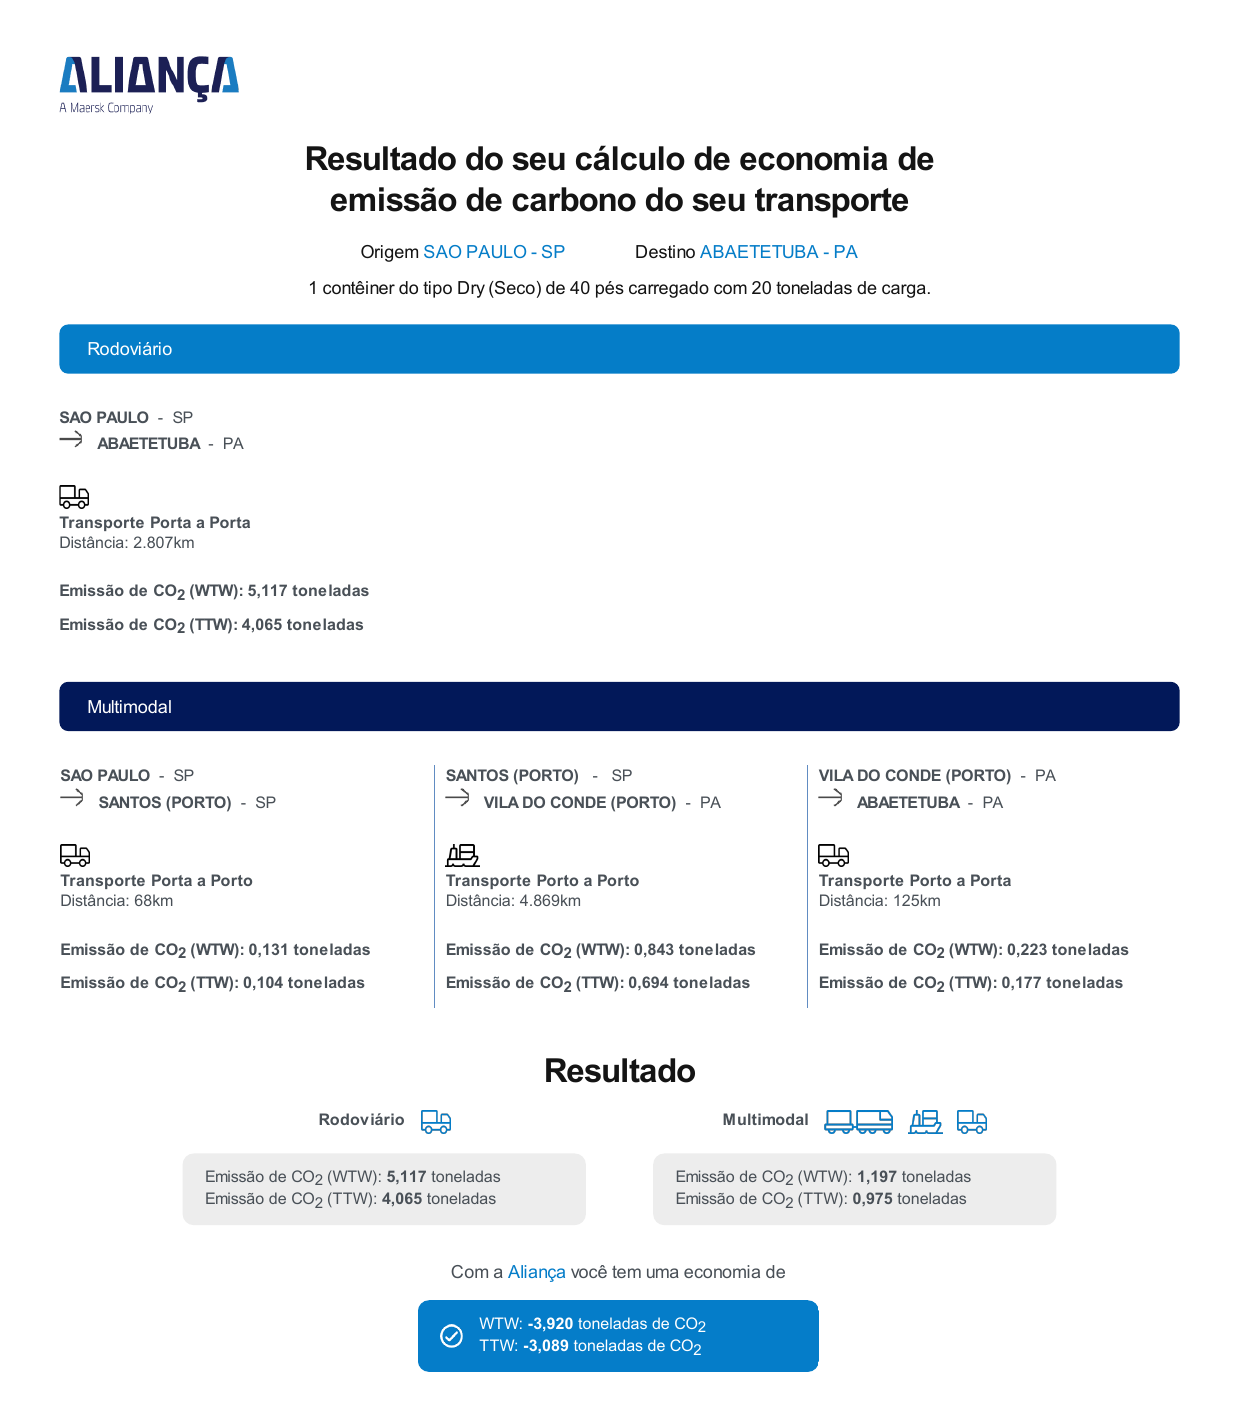
\includegraphics[width=0.94\linewidth]{comparacao_externa/calculo-co2_86072221.png}
\end{center}

\emph{Figura 10 --- Resultado da calculadora da Aliança para São
Paulo--Abaetetuba. Fonte: resultado exportado pela ferramenta, fornecido
pelo autor.}

\textbf{Tabela 19 --- Emissões TTW por etapa no cenário São
Paulo--Abaetetuba, com 20 t de carga.}

\begin{longtable}[]{@{}lrrrr@{}}
\toprule
\begin{minipage}[b]{0.17\columnwidth}\raggedright
Etapa\strut
\end{minipage} & \begin{minipage}[b]{0.17\columnwidth}\raggedleft
Aliança: distância\strut
\end{minipage} & \begin{minipage}[b]{0.17\columnwidth}\raggedleft
Aliança: CO\textsubscript{2} TTW\strut
\end{minipage} & \begin{minipage}[b]{0.17\columnwidth}\raggedleft
CabotageLens: distância\strut
\end{minipage} & \begin{minipage}[b]{0.17\columnwidth}\raggedleft
CabotageLens: CO\textsubscript{2}e TTW\strut
\end{minipage}\tabularnewline
\midrule
\endhead
\begin{minipage}[t]{0.17\columnwidth}\raggedright
Rodovia direta\strut
\end{minipage} & \begin{minipage}[t]{0.17\columnwidth}\raggedleft
2.807 km\strut
\end{minipage} & \begin{minipage}[t]{0.17\columnwidth}\raggedleft
4,065 t\strut
\end{minipage} & \begin{minipage}[t]{0.17\columnwidth}\raggedleft
2.835,762 km\strut
\end{minipage} & \begin{minipage}[t]{0.17\columnwidth}\raggedleft
3,800 t\strut
\end{minipage}\tabularnewline
\begin{minipage}[t]{0.17\columnwidth}\raggedright
Acesso rodoviário inicial: São Paulo--Santos\strut
\end{minipage} & \begin{minipage}[t]{0.17\columnwidth}\raggedleft
68 km\strut
\end{minipage} & \begin{minipage}[t]{0.17\columnwidth}\raggedleft
0,104 t\strut
\end{minipage} & \begin{minipage}[t]{0.17\columnwidth}\raggedleft
86,170 km\strut
\end{minipage} & \begin{minipage}[t]{0.17\columnwidth}\raggedleft
0,115 t\strut
\end{minipage}\tabularnewline
\begin{minipage}[t]{0.17\columnwidth}\raggedright
Navegação: Santos--Vila do Conde\strut
\end{minipage} & \begin{minipage}[t]{0.17\columnwidth}\raggedleft
4.869 km\strut
\end{minipage} & \begin{minipage}[t]{0.17\columnwidth}\raggedleft
0,694 t\strut
\end{minipage} & \begin{minipage}[t]{0.17\columnwidth}\raggedleft
4.495,000 km\strut
\end{minipage} & \begin{minipage}[t]{0.17\columnwidth}\raggedleft
0,918 t\strut
\end{minipage}\tabularnewline
\begin{minipage}[t]{0.17\columnwidth}\raggedright
Operações portuárias: Santos e Vila do Conde\strut
\end{minipage} & \begin{minipage}[t]{0.17\columnwidth}\raggedleft
---\strut
\end{minipage} & \begin{minipage}[t]{0.17\columnwidth}\raggedleft
Não discriminadas\strut
\end{minipage} & \begin{minipage}[t]{0.17\columnwidth}\raggedleft
---\strut
\end{minipage} & \begin{minipage}[t]{0.17\columnwidth}\raggedleft
0,026 t\strut
\end{minipage}\tabularnewline
\begin{minipage}[t]{0.17\columnwidth}\raggedright
Acesso rodoviário final: Vila do Conde--Abaetetuba\strut
\end{minipage} & \begin{minipage}[t]{0.17\columnwidth}\raggedleft
125 km\strut
\end{minipage} & \begin{minipage}[t]{0.17\columnwidth}\raggedleft
0,177 t\strut
\end{minipage} & \begin{minipage}[t]{0.17\columnwidth}\raggedleft
33,950 km\strut
\end{minipage} & \begin{minipage}[t]{0.17\columnwidth}\raggedleft
0,045 t\strut
\end{minipage}\tabularnewline
\begin{minipage}[t]{0.17\columnwidth}\raggedright
\textbf{Total multimodal}\strut
\end{minipage} & \begin{minipage}[t]{0.17\columnwidth}\raggedleft
\textbf{5.062 km}\strut
\end{minipage} & \begin{minipage}[t]{0.17\columnwidth}\raggedleft
\textbf{0,975 t}\strut
\end{minipage} & \begin{minipage}[t]{0.17\columnwidth}\raggedleft
\textbf{4.615,120 km}\strut
\end{minipage} & \begin{minipage}[t]{0.17\columnwidth}\raggedleft
\textbf{1,104 t}\strut
\end{minipage}\tabularnewline
\begin{minipage}[t]{0.17\columnwidth}\raggedright
\textbf{Redução em relação à rodovia direta}\strut
\end{minipage} & \begin{minipage}[t]{0.17\columnwidth}\raggedleft
---\strut
\end{minipage} & \begin{minipage}[t]{0.17\columnwidth}\raggedleft
\textbf{3,090 t (76,0\%)}\strut
\end{minipage} & \begin{minipage}[t]{0.17\columnwidth}\raggedleft
---\strut
\end{minipage} & \begin{minipage}[t]{0.17\columnwidth}\raggedleft
\textbf{2,696 t (70,9\%)}\strut
\end{minipage}\tabularnewline
\bottomrule
\end{longtable}

Na rodovia direta, as distâncias são próximas: 2.807 km na Aliança e
2.835,762 km no CabotageLens. Na cadeia multimodal, a Aliança informa
4.869 km para a navegação e 125 km para o acesso final, enquanto o
CabotageLens usa 4.495 km e 33,950 km, respectivamente. A diferença
restante decorre sobretudo do acesso final e da referência de distância
adotada para cada porto.

A distância total multimodal soma apenas os dois acessos rodoviários e a
etapa marítima; as operações portuárias não acrescentam distância. A
Aliança não as separa: os três trechos exibidos pela ferramenta somam
exatamente o total multimodal de 0,975 t. No CabotageLens, essas
operações aparecem como uma etapa própria, com 0,026 t de CO\textsubscript{2}e TTW, e
são incluídas no total. A tabela compara apenas TTW, que é o escopo
adotado pelo CabotageLens; a calculadora da Aliança também exibe valores
WTW, mas eles não são usados nesta comparação.

Há uma inconsistência de sinal no quadro de economia exibido pela
Aliança: a diferença entre seus próprios totais TTW é aproximadamente
4,065 − 0,975 = 3,090 t de redução, mas a tela apresenta −3,089 t. Por
esse motivo, a última linha da tabela é calculada diretamente a partir
dos totais de cada alternativa. O CabotageLens apresenta a redução com
sinal coerente com as emissões totais mostradas.

\hypertarget{calculadora-de-emissuxf5es-da-log-in}{%
\subsection{\texorpdfstring{5.2
\href{https://www.loginlogistica.com.br/calculadora-co2/}{Calculadora de
emissões da
Log-In}}{5.2 Calculadora de emissões da Log-In}}\label{calculadora-de-emissuxf5es-da-log-in}}

A captura da calculadora da Log-In \parencite{login2026} refere-se ao cenário São Paulo--Rio
Branco e mostra uma alternativa rodoviária de 3.032 km. A alternativa
por cabotagem é composta por três trechos de 89,9 km, 6.112 km e 1.394
km, compatíveis com a estrutura São Paulo--Santos--Manaus--Rio Branco. O
mesmo cenário foi executado no CabotageLens com 14 t e 1 TEU.

\begin{center}
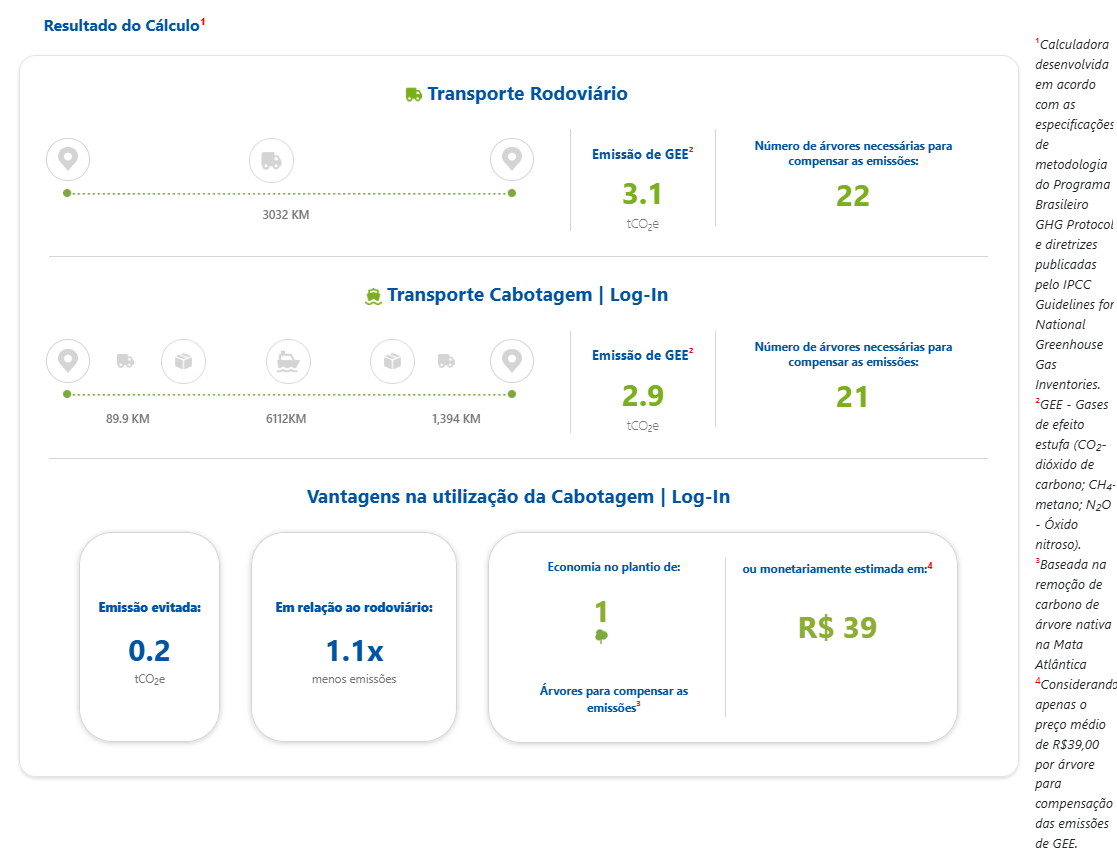
\includegraphics[width=0.94\linewidth]{comparacao_externa/loginlogistica.png}
\end{center}

\emph{Figura 11 --- Resultado da calculadora de emissões da Log-In.
Fonte: captura de tela fornecida pelo autor.}

\textbf{Tabela 20 --- Emissões no cenário de referência São Paulo--Rio
Branco.}

\begin{longtable}[]{@{}lrrrr@{}}
\toprule
\begin{minipage}[b]{0.17\columnwidth}\raggedright
Alternativa\strut
\end{minipage} & \begin{minipage}[b]{0.17\columnwidth}\raggedleft
Log-In: distância\strut
\end{minipage} & \begin{minipage}[b]{0.17\columnwidth}\raggedleft
Log-In: emissões de GEE\strut
\end{minipage} & \begin{minipage}[b]{0.17\columnwidth}\raggedleft
CabotageLens: distância\strut
\end{minipage} & \begin{minipage}[b]{0.17\columnwidth}\raggedleft
CabotageLens: CO\textsubscript{2}e TTW\strut
\end{minipage}\tabularnewline
\midrule
\endhead
\begin{minipage}[t]{0.17\columnwidth}\raggedright
Rodovia direta\strut
\end{minipage} & \begin{minipage}[t]{0.17\columnwidth}\raggedleft
3.032 km\strut
\end{minipage} & \begin{minipage}[t]{0.17\columnwidth}\raggedleft
3,1 t\strut
\end{minipage} & \begin{minipage}[t]{0.17\columnwidth}\raggedleft
3.491,431 km\strut
\end{minipage} & \begin{minipage}[t]{0.17\columnwidth}\raggedleft
4,068 t\strut
\end{minipage}\tabularnewline
\begin{minipage}[t]{0.17\columnwidth}\raggedright
Multimodal\strut
\end{minipage} & \begin{minipage}[t]{0.17\columnwidth}\raggedleft
7.595,9 km\strut
\end{minipage} & \begin{minipage}[t]{0.17\columnwidth}\raggedleft
2,9 t\strut
\end{minipage} & \begin{minipage}[t]{0.17\columnwidth}\raggedleft
7.584,836 km\strut
\end{minipage} & \begin{minipage}[t]{0.17\columnwidth}\raggedleft
3,042 t\strut
\end{minipage}\tabularnewline
\begin{minipage}[t]{0.17\columnwidth}\raggedright
Redução em relação à rodovia\strut
\end{minipage} & \begin{minipage}[t]{0.17\columnwidth}\raggedleft
---\strut
\end{minipage} & \begin{minipage}[t]{0.17\columnwidth}\raggedleft
0,2 t\strut
\end{minipage} & \begin{minipage}[t]{0.17\columnwidth}\raggedleft
---\strut
\end{minipage} & \begin{minipage}[t]{0.17\columnwidth}\raggedleft
1,027 t\strut
\end{minipage}\tabularnewline
\bottomrule
\end{longtable}

No resultado multimodal, as duas ferramentas estão próximas. A distância
da Log-In é 11,064 km maior, uma diferença de 0,15\%, e a emissão de GEE
informada é 0,142 t menor, ou 4,7\% em relação ao CabotageLens. Essa
proximidade é positiva porque os valores divulgados pelas duas
ferramentas são semelhantes, mesmo usando fontes e parâmetros próprios.

Na alternativa rodoviária, porém, a distância da Log-In não corresponde
à rota porta a porta São Paulo--Rio Branco previamente calculada. A
ferramenta informa 3.032 km, enquanto o CabotageLens obteve 3.491,431 km
e a conferência independente no Google Maps indicou 3.497 km, como
apresentado na Seção 4.3.1.1. Essa diferença de 459,431 km, ou 13,2\%,
contribui para que a emissão rodoviária informada pela Log-In seja
menor. Por isso, a comparação rodoviária não deve ser interpretada como
uma equivalência direta entre os dois sistemas.

\hypertarget{calculadora-de-piso-muxednimo-de-frete-da-antt}{%
\subsection{\texorpdfstring{5.3
\href{https://calculadorafrete.antt.gov.br/}{Calculadora de piso mínimo
de frete da
ANTT}}{5.3 Calculadora de piso mínimo de frete da ANTT}}\label{calculadora-de-piso-muxednimo-de-frete-da-antt}}

Na calculadora da Agência Nacional de Transportes Terrestres (ANTT)
\parencite{anttfrete2026}, o
cenário foi informado como carga conteinerizada, cinco eixos e 3.491 km.
O resultado oficial exibido foi R\$ 21.308,12. Para a mesma ligação São
Paulo--Rio Branco, o CabotageLens calculou 3.491,431 km, selecionou
cinco eixos para a carga de 14 t e estimou R\$ 12.318,68 de custo de
combustível.

\begin{center}
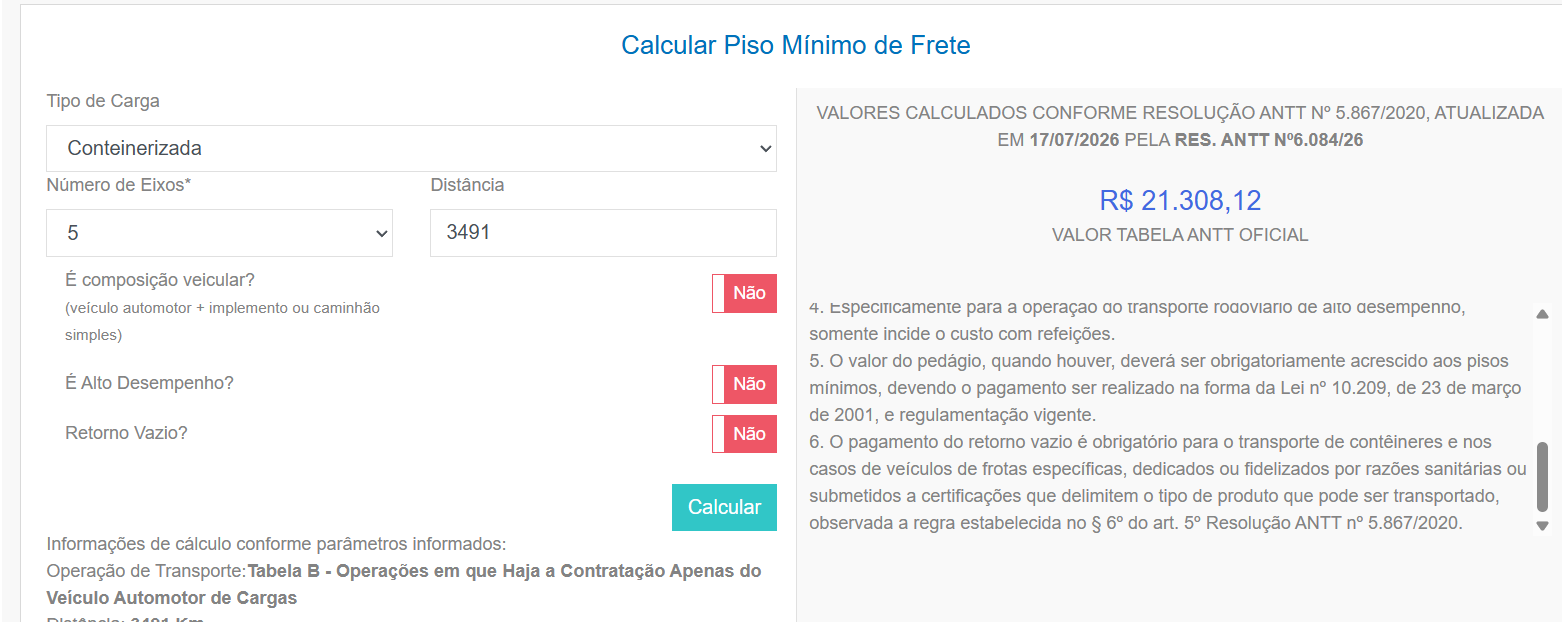
\includegraphics[width=0.94\linewidth]{comparacao_externa/calculadorafreteantt.png}
\end{center}

\emph{Figura 12 --- Resultado da calculadora de piso mínimo de frete da
ANTT para a distância de 3.491 km. Fonte: captura de tela fornecida pelo
autor.}

\textbf{Tabela 21 --- Valores para a ligação São Paulo--Rio Branco.}

\begin{longtable}[]{@{}lrr@{}}
\toprule
\begin{minipage}[b]{0.30\columnwidth}\raggedright
Item\strut
\end{minipage} & \begin{minipage}[b]{0.30\columnwidth}\raggedleft
Calculadora da ANTT\strut
\end{minipage} & \begin{minipage}[b]{0.30\columnwidth}\raggedleft
CabotageLens\strut
\end{minipage}\tabularnewline
\midrule
\endhead
\begin{minipage}[t]{0.30\columnwidth}\raggedright
Distância\strut
\end{minipage} & \begin{minipage}[t]{0.30\columnwidth}\raggedleft
3.491 km\strut
\end{minipage} & \begin{minipage}[t]{0.30\columnwidth}\raggedleft
3.491,431 km\strut
\end{minipage}\tabularnewline
\begin{minipage}[t]{0.30\columnwidth}\raggedright
Configuração do veículo\strut
\end{minipage} & \begin{minipage}[t]{0.30\columnwidth}\raggedleft
5 eixos\strut
\end{minipage} & \begin{minipage}[t]{0.30\columnwidth}\raggedleft
5 eixos\strut
\end{minipage}\tabularnewline
\begin{minipage}[t]{0.30\columnwidth}\raggedright
Valor calculado\strut
\end{minipage} & \begin{minipage}[t]{0.30\columnwidth}\raggedleft
R\$ 21.308,12 --- piso mínimo de frete\strut
\end{minipage} & \begin{minipage}[t]{0.30\columnwidth}\raggedleft
R\$ 12.318,68 --- custo modelado do combustível\strut
\end{minipage}\tabularnewline
\bottomrule
\end{longtable}

Os dois valores têm finalidades diferentes: o resultado da ANTT é o piso
mínimo de frete, enquanto o CabotageLens isola o custo operacional de
combustível. Por isso, não se espera que sejam iguais. Ainda assim, o
combustível calculado pelo sistema, R\$~12.318,68, representa 57,8\% do
piso de R\$~21.308,12. Essa proporção é um sinal de coerência de ordem
de grandeza, pois o piso mínimo também reúne outras parcelas do frete
além do combustível. Assim, os valores são apresentados lado a lado para
contextualização, e não como cotações equivalentes.

\clearpage
\hypertarget{conclusuxf5es}{%
\section{6. Conclusões}\label{conclusuxf5es}}

\hypertarget{resultados-da-comparauxe7uxe3o}{%
\subsection{6.1 Resultados da
comparação}\label{resultados-da-comparauxe7uxe3o}}

Este trabalho apresentou o CabotageLens, uma ferramenta para comparar
duas formas de transportar a mesma remessa entre uma origem e um
destino: a alternativa rodoviária direta e a alternativa multimodal com
acessos rodoviários, operações portuárias e cabotagem. Ao aplicar as
duas alternativas à mesma carga, origem e destino, o sistema evita
comparar apenas o trecho marítimo com uma viagem rodoviária completa.

No exemplo de uma remessa de 14~t entre São Paulo e Rio Branco, a
alternativa multimodal percorre 117,24\% mais quilômetros do que a
rodoviária direta. Mesmo assim, emite 25,24\% menos CO\textsubscript{2}e operacional e
apresenta custo modelado do combustível 43,84\% menor. O resultado
mostra que a distância total, isoladamente, não é suficiente para
comparar os modais: os acessos rodoviários, as operações portuárias e a
navegação precisam ser avaliados na mesma cadeia logística.

\hypertarget{contribuiuxe7uxe3o-metodoluxf3gica}{%
\subsection{6.2 Contribuição
metodológica}\label{contribuiuxe7uxe3o-metodoluxf3gica}}

A principal contribuição do CabotageLens está na construção da perna
marítima com dados observados. Em vez de fixar um corredor entre dois
portos, o sistema reconstrói as viagens registradas pela Agência
Nacional de Transportes Aquaviários (ANTAQ), preserva as escalas
intermediárias e calcula a carga a bordo em cada subtrecho. Sempre que
possível, a intensidade vem do mesmo número IMO na base europeia de
Monitoramento, Reporte e Verificação da União Europeia (EU MRV). Quando
essa correspondência não está disponível ou é considerada atípica, o
cálculo usa uma referência estatística de navios semelhantes e informa a
fonte adotada.

A ligação Santos--Manaus demonstra o efeito dessa escolha: os 89
recortes completos formam 22 sequências de portos, com viagens diretas e
viagens com escalas intermediárias. Para a distância, os 2 recortes acima
do P95 de 6.975,000~km são retirados da média, resultando em
6.094,975~km com 87 recortes; a intensidade de 9,009824~g/(t·nm)
continua usando os 89 recortes. Portanto, esses indicadores não
descrevem uma rota única nem o desempenho de um único navio; sua
procedência permanece registrada para conferência.

Além da contribuição metodológica, o CabotageLens constitui uma
contribuição aplicada e acessível: a
\href{https://cabotagelens.streamlit.app/}{aplicação está disponível
publicamente} e seu
\href{https://github.com/pennylanesccp/cabotage-lens}{código-fonte,
documentação e regras de cálculo podem ser consultados no repositório
público do projeto}. Dessa forma, outras pessoas podem executar cenários
próprios, conferir as premissas adotadas e reproduzir a lógica de cálculo,
dentro dos limites de dados e escopo descritos neste trabalho.

\clearpage
\begingroup
\small
\printbibliography[heading=bibintoc,title={Referências}]
\endgroup

\end{document}
